\documentclass{article}
\usepackage[utf8]{inputenc}
\usepackage{lscape}
\usepackage{pdflscape}
\usepackage{longtable}
\usepackage{amsfonts, amsmath, amssymb,array,comment}
\usepackage[round]{natbib}
\usepackage{soul}
\usepackage{float,graphicx}

\usepackage{footnote}
\usepackage[flushleft]{threeparttable}
\usepackage{threeparttablex}
\makesavenoteenv{tabular}
\makesavenoteenv{table}
\newcommand*{\id}{{\normalfont\hbox{1\kern-0.15em \vrule width .8pt depth-.5pt}}}

\usepackage{tikz}
\usetikzlibrary{shapes}
\usetikzlibrary{fit}
\usetikzlibrary{chains}
\usetikzlibrary{arrows}
% Latent node
\tikzstyle{latent} = [circle,fill=white,draw=black,inner sep=1pt,
minimum size=20pt, font=\fontsize{10}{10}\selectfont, node distance=1]
% Observed node
\tikzstyle{obs} = [latent,fill=gray!25]
% Marginal node
\tikzstyle{margin} = [latent,dashed,draw=gray!40!black]
% Constant node
\tikzstyle{const} = [rectangle, inner sep=1pt, node distance=1]
\tikzstyle{parameter} = [rectangle, inner sep=0pt, node distance=1]
% Factor node
\tikzstyle{factor} = [rectangle, fill=black,minimum size=5pt, inner
sep=0pt, node distance=0.4]
% Deterministic node
\tikzstyle{det} = [latent, diamond]

% Plate node
\tikzstyle{plate} = [draw, rectangle, rounded corners, fit=#1]
% Invisible wrapper node
\tikzstyle{wrap} = [inner sep=0pt, fit=#1]
% Gate
\tikzstyle{gate} = [draw, rectangle, dashed, fit=#1]

% Caption node
\tikzstyle{caption} = [font=\footnotesize, node distance=0] %
\tikzstyle{plate caption} = [caption, node distance=0, inner sep=0pt,
below left=5pt and 0pt of #1.south east] %
\tikzstyle{factor caption} = [caption] %
\tikzstyle{every label} += [caption] %

\tikzset{>={triangle 45}}

%\pgfdeclarelayer{b}
%\pgfdeclarelayer{f}
%\pgfsetlayers{b,main,f}

% \factoredge [options] {inputs} {factors} {outputs}
\newcommand{\factoredge}[4][]{ %
  % Connect all nodes #2 to all nodes #4 via all factors #3.
  \foreach \f in {#3} { %
    \foreach \x in {#2} { %
      \path (\x) edge[-,#1] (\f) ; %
      %\draw[-,#1] (\x) edge[-] (\f) ; %
    } ;
    \foreach \y in {#4} { %
      \path (\f) edge[->,#1] (\y) ; %
      %\draw[->,#1] (\f) -- (\y) ; %
    } ;
  } ;
}

% \edge [options] {inputs} {outputs}
\newcommand{\edge}[3][]{ %
  % Connect all nodes #2 to all nodes #3.
  \foreach \x in {#2} { %
    \foreach \y in {#3} { %
      \path (\x) edge [->,#1] (\y) ;%
      %\draw[->,#1] (\x) -- (\y) ;%
    } ;
  } ;
}

% \factor [options] {name} {caption} {inputs} {outputs}
\newcommand{\factor}[5][]{ %
  % Draw the factor node. Use alias to allow empty names.
  \node[factor, label={[name=#2-caption]#3}, name=#2, #1,
  alias=#2-alias] {} ; %
  % Connect all inputs to outputs via this factor
  \factoredge {#4} {#2-alias} {#5} ; %
}

% \plate [options] {name} {fitlist} {caption}
\newcommand{\plate}[4][]{ %
  \node[wrap=#3] (#2-wrap) {}; %
  \node[plate caption=#2-wrap] (#2-caption) {#4}; %
  \node[plate=(#2-wrap)(#2-caption), #1] (#2) {}; %
}

% \gate [options] {name} {fitlist} {inputs}
\newcommand{\gate}[4][]{ %
  \node[gate=#3, name=#2, #1, alias=#2-alias] {}; %
  \foreach \x in {#4} { %
    \draw [-*,thick] (\x) -- (#2-alias); %
  } ;%
}

% \vgate {name} {fitlist-left} {caption-left} {fitlist-right}
% {caption-right} {inputs}
\newcommand{\vgate}[6]{ %
  % Wrap the left and right parts
  \node[wrap=#2] (#1-left) {}; %
  \node[wrap=#4] (#1-right) {}; %
  % Draw the gate
  \node[gate=(#1-left)(#1-right)] (#1) {}; %
  % Add captions
  \node[caption, below left=of #1.north ] (#1-left-caption)
  {#3}; %
  \node[caption, below right=of #1.north ] (#1-right-caption)
  {#5}; %
  % Draw middle separation
  \draw [-, dashed] (#1.north) -- (#1.south); %
  % Draw inputs
  \foreach \x in {#6} { %
    \draw [-*,thick] (\x) -- (#1); %
  } ;%
}

% \hgate {name} {fitlist-top} {caption-top} {fitlist-bottom}
% {caption-bottom} {inputs}
\newcommand{\hgate}[6]{ %
  % Wrap the left and right parts
  \node[wrap=#2] (#1-top) {}; %
  \node[wrap=#4] (#1-bottom) {}; %
  % Draw the gate
  \node[gate=(#1-top)(#1-bottom)] (#1) {}; %
  % Add captions
  \node[caption, above right=of #1.west ] (#1-top-caption)
  {#3}; %
  \node[caption, below right=of #1.west ] (#1-bottom-caption)
  {#5}; %
  % Draw middle separation
  \draw [-, dashed] (#1.west) -- (#1.east); %
  % Draw inputs
  \foreach \x in {#6} { %
    \draw [-*,thick] (\x) -- (#1); %
  } ;%
}

\usepackage{hyperref}
\hypersetup{
    colorlinks,
    citecolor=black,
    linktoc=all,
    filecolor=blue,
    linkcolor=black,
    urlcolor=black
}

%\pagenumbering{gobble} %% suppresses page numbers
\usepackage[left=2cm, right=2cm, top=2cm, bottom=2cm]{geometry}
\title{ITHIM}

\begin{document}
\maketitle
\tableofcontents
\clearpage
\section{Introduction}

\subsection{Summary of literature}

\subsection{Summary of aims}

\subsection{Overview}

The remainder of the document presents a current working version of the ITHIM, and is a comprehensive record of all the calculations of which it is composed. The equations for the ITHIM are described in Section \ref{equations} (tabulated in Section \ref{tableequations}). The method is concretised through the example application to Accra in Section \ref{example} and particular columns in Tables \ref{indices} and \ref{inputs}, with results presented in Section \ref{results}. 

The ITHIM as described here is implemented in the ITHIM-R R package (\url{https://github.com/ITHIM/ITHIM-R}). Other cities are also included in that package (S\~{a}o Paulo, Delhi, Bangalore), and reference will be made to those where relevant.
% Some details here are specific to the Accra version of that model, as Accra has been the setting for construction of the prototype. 

\section{Method: ITHIM}\label{equations}

In the ITHIM, we combine many information inputs and compute the health burden through three pathways (depicted in Figure \ref{workflow}). Each pathway has its own set of definitions and outputs, and we refer to them as ``modules''.

\begin{figure}[h]
  \centering
  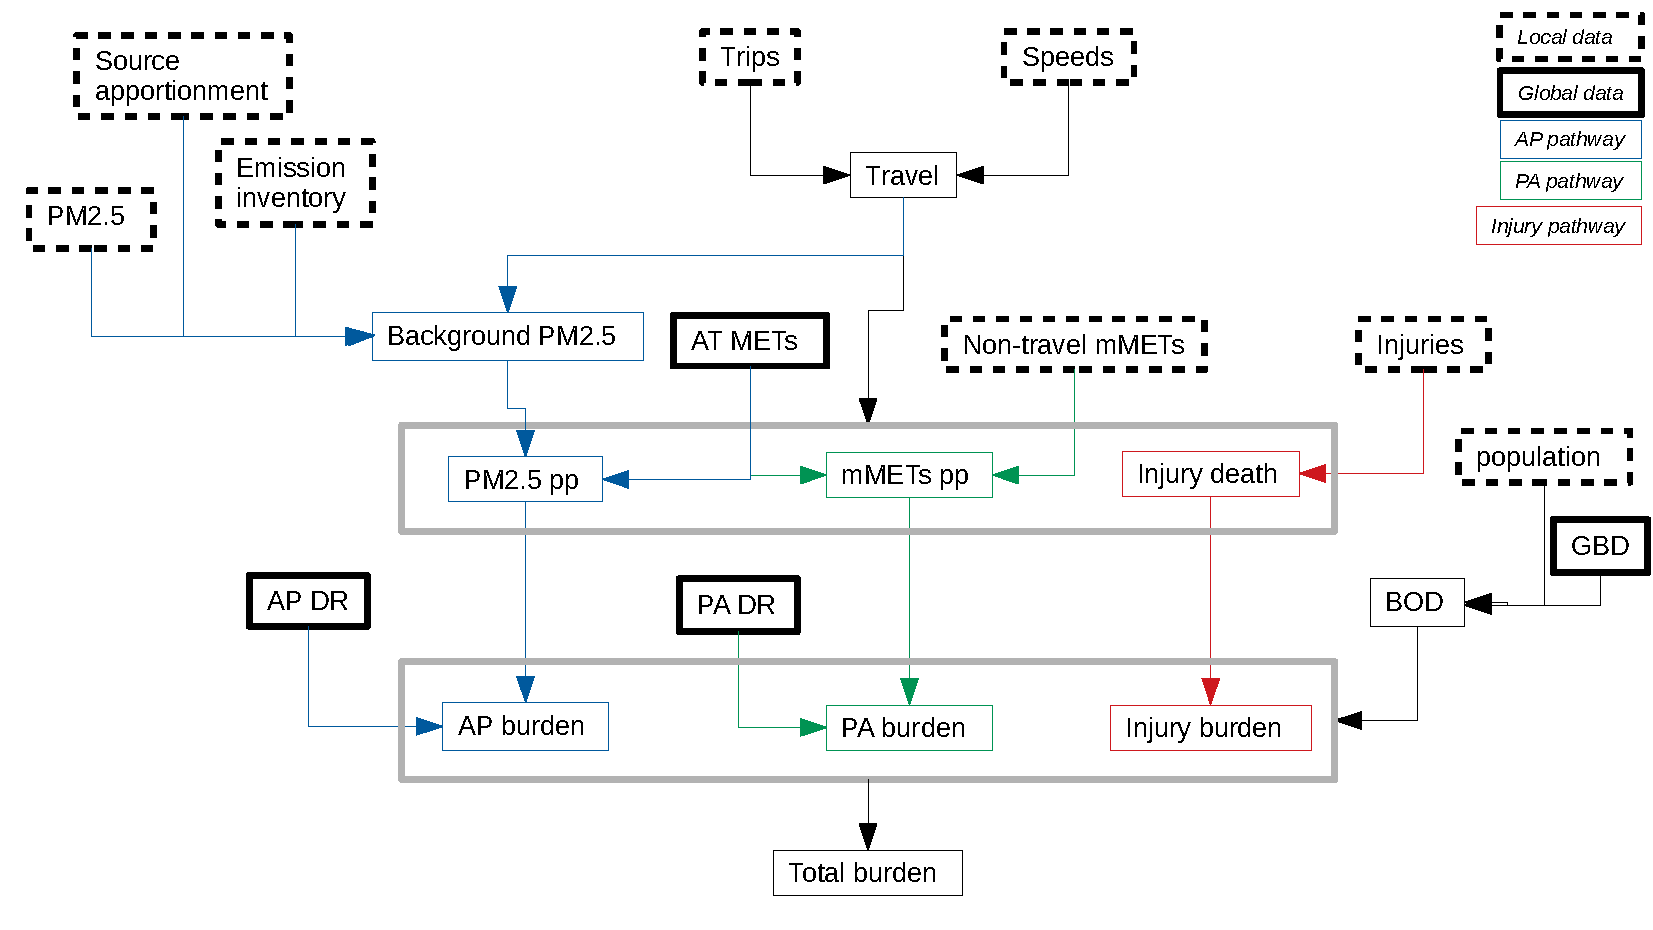
\includegraphics[width=0.9\textwidth]{flowchart.pdf}
  \caption{\small ITHIM workflow. Inputs to the model have a bold, black outline. The graph depicts parent--child relationships, where a child (at the head of an arrow) depends upon all its parents (at the source(s) of the arrow(s)). To aid visualisation, an arrow connected to the outside of a grey box indicates that the arrow connects to each item within the box. \textit{AT: active travel. MET: metabolic equivalent task. pp: per person. AP: air pollution. PA: physical activity. DR: dose--response relationship. GBD: global burden of disease. BOD: (local) burden of disease.}}
\label{workflow}
\end{figure}

To describe the model, we use lower-case letters to denote indices, or dimensions, of objects. They take one of a set of possible values, detailed in Table \ref{indices}. The set of input items are denoted by capital letters, and variable parameters are denoted by Greek letters. These are presented in Table \ref{inputs}. The equations of the ITHIM are presented below, and summarised in Table \ref{calculationstab}. These use letter modifiers to show how the inputs are modified in the course of output generation. %A description of the dose--response relationship parametrisation is given in Section \ref{dr}.

We calculate the ITHIM by combining the modules' outputs in terms of the health burden ($\hat{U}_{a,g,h,o,s}$). Other outputs of the model include: MMETs per person ($M_{i,s}$), PM2.5 in each scenario ($\bar{P}_s$), PM2.5 per person ($\check{W}_{i,s}$), and injuries burden ($\check{I}_{a,g,m,o,s}$).

To assess uncertainty, we sample from the ITHIM output by sampling uncertain parameters multiple times and calculating the ITHIM. We specify parametric distributions or sampling strategies for all the uncertain parameters. Evaluating the ITHIM with uncertain parameters allows assessment of their impact on the outcome (AKA sensitivity analysis). We use EVPPI to calculate the expected reduction in uncertainty in the outcome were we to learn a parameter perfectly. This means we can implement models that are basic in their parametrisation, and learn at the end for which parameters it would be worthwhile spending dedicated time learning better. 


\begin{table}[ht]
\begin{center}
\caption{\small Indices used in the ITHIM variables. The ``Label'' is the subscript used to refer to the index in this document. The ``Name'' is descriptive. The ``Levels'' are the levels used in the Accra model.}
\begin{tabular}{lll}
\label{indices}
Label & Name & Levels  \\
\hline
$a$ & Age group & 15--49 \\
&  & 50--69  \\
$g$ & Gender & Male \\
&  & Female  \\
$h$ & Disease &  \\
$i$ & Individual index &  \\
$j$ & Trip index & \\
$m$ & Transport mode& walk  \\
&& cycling (cyc.)  \\
&& bus \\
&& car  \\
&& motorbike (mot.)  \\
&& goods vehicles (GV)  \\
&& subway (sub.)  \\
$o$ & Outcome & Death  \\
& & YLL  \\
%$p$ & PM2.5 levels \\
$s$ & Scenario & \\
$w$ & AP RR hyperparameter & $1,2,3,4$ \\
$x$ & PA RR hyperparameter & $1,2,3$ \\
$z$ & PA dose & $0,...,300$ \\
\hline
\end{tabular}
\end{center}
\end{table}

\begin{table}[ht]
\begin{center}
\caption{\small Common abbreviations.}
\begin{tabular}{ll}
\label{abbrev}
Abbreviation & Meaning  \\
\hline
AP & Air pollution \\
CDF & Cumulative distribution function \\
COPD & Chronic obstructive pulmonary disease \\
DR & Dose response \\
EVPPI & Expected value of perfect partial information \\
GAM & Generalised additive model \\
GBD & Global burden of disease\\
IHD & Ischemic heart disease\\
ITHIM & Integrated transport and health impact model \\
LRI & Lower respiratory infection \\
MMET & Marginal metabolic equivalent task \\
PA & Physical activity\\
PAF & Population attributable fraction\\
PIF & Potential impact fraction\\
PM2.5 & Particulate matter (diameter $< 2.5 \mu$m)\\
PT & Public transport\\
RR & Relative risk \\
VOI & Value of information \\
YLL & Years of life lost \\
\hline
\end{tabular}
\end{center}
\end{table}

\begin{landscape}

\begin{center}
\begin{longtable}{lp{5cm}|lrr}
\caption{\small All values input to the ITHIM model.}\\
\label{inputs}
&&\multicolumn{3}{r}{\textit{ITHIM-R reference}}\\

Name & Description & Value in Accra model & Label & Model/ Setting\\

\hline
\multicolumn{2}{l|}{\textit{Global values}}&&&\\
\hline
$U_{a,g,h,o}$ & Background burden of disease   & Constant & GBD\_DATA &  Setting \\

$N_{a,g}$ & Population by age and gender in GBD\_DATA & Constant & GBD\_DATA & Setting \\



$\bar{N}_{a,g}$ & Population by age and gender & Constant & DEMOGRAPHIC & Setting \\

$\rho_h$ & Chronic disease scalar & 1 or Lnorm(0,0.18) & CHRONIC\_DISEASE\_SCALAR & Setting \\ 
\hline
\multicolumn{2}{l|}{\textit{Travel values}}\\
\hline

$Z_{m=walk}$ & Walk speed & 4.8 & MODE\_SPEEDS &  Setting \\
$Z_{m=cyc.}$ & Cycle speed & 14.5 & MODE\_SPEEDS  & Setting \\
$Z_{m=bus}$ & Bus speed & 15 & MODE\_SPEEDS & Setting \\
$Z_{m=car}$ & Car speed & 21 & MODE\_SPEEDS &  Setting \\
$Z_{m=mot.}$ & Motorbike speed & 25 & MODE\_SPEEDS  & Setting \\
 
$\epsilon$ & Walk time to bus & 5 or Lnorm(log(5),0.18) & BUS\_WALK\_TIME &  Setting \\

%$\mu_{m=mot.}$ & Motorcycle distance relative to car & 0.2 or Lnorm(-1.4,0.4) & MOTORCYCLE\_TO\_CAR\_RATIO &  & Setting \\

$\mu_{m=HGV}$ & Truck distance relative to car & 0.21 or Beta(3,10) & TRUCK\_TO\_CAR\_RATIO &  Setting \\

$\mu_{m=bus}$ & Bus driver distance relative to bus passenger distance & 1/45 or Beta(20,600) & BUS\_TO\_PASSENGER\_RATIO & Setting \\

$\mu_{m=mot.}$ & Motorcycle fleet distance relative to total motorcycle distance & 37/68 or Beta(37/3+1,31/3+1) & FLEET\_TO\_MOTORCYCLE\_RATIO & Setting \\

$T_j$ & Trip-level data & Constant & SYNTHETIC\_TRIPS &    Setting\\

%$Q_i$ & Person weights & Constant (1) & SYNTHETIC\_POPULATION\$ weight (TBI) &   & Setting\\

\hline
\multicolumn{2}{l|}{\textit{Injury model values}}\\
\hline

$I_{a,g,m_{\text{vic}},m_{\text{str}}}$ & Fatalities table & Constant & INJURY\_TABLE &   Setting\\

$\sigma$ & Injury reporting rate & 1 or Beta(8,3) & INJURY\_REPORTING\_RATE &  Setting \\ 

$\omega$ & Sum of distance exponents & 1.9 or Lnorm(log(1.9),log(1.03)) & SIN\_EXPONENT\_SUM & Model \\

$\psi$ & Casualty fraction of $\omega$  & 0.5 or Beta(20,20) & CASUALTY\_EXPONENT\_ FRACTION &  Model \\

\hline
\multicolumn{2}{l|}{\textit{Pollution model values}}\\
\hline

$\eta$ & {Background PM2.5 concentration} & 50 or Lnorm(log(50),0.18) &PM\_CONC\_BASE&  Setting\\
$\zeta$ & Fraction of measured PM2.5 concentration due to road transport & 0.225 or Beta(5,20) & PM\_TRANS\_SHARE &   Setting\\

$\gamma_{m}$ & Vehicle emission inventory  & Constant or Dirichlet & EMISSION\_INVENTORY & Setting \\

$P$ & Vehicle emission confidence  & 1 & EMISSION\_INVENTORY\_CONFIDENCE & Setting \\

\hline
\multicolumn{2}{l|}{\textit{Pollution \& health model values}}\\
\hline

$C_1$ & Base-level inhalation rate & 1 & BASE\_LEVEL\_INHALATION \_RATE &   Model \\
$C_2$ & Exposure ratio window closed & 0.5 & CLOSED\_WINDOW\_PM\_ RATIO &   Model \\
$C_3$ & Proportion of travel with closed windows & 0.5 & CLOSED\_WINDOW\_RATIO   & Setting \\
$C_4$ & Parameter for on-road PM2.5 level & 3.216 & ROAD\_RATIO\_MAX   & Model \\
$C_5$ & Parameter for on-road PM2.5 level & 0.379 & ROAD\_RATIO\_SLOPE  & Model \\
$C_6$ & Exposure ratio for underground & 0.8 & SUBWAY\_PM\_RATIO &  Setting \\

$H_{a,h,w}$ & {AP dose--response--curve parameters} & Constant & DR\_AP  & Model\\

$\xi_{h,w}$ & Quantiles for AP RR functions & 0.5 or Unif(0,1) & AP\_DOSE\_RESPONSE\_ QUANTILE &   Model\\

\hline
\multicolumn{2}{l|}{\textit{Physical activity model values}}\\
\hline
$\chi$ & Day-to-week travel scalar & 7 or 7$\times$Beta(20,3) & DAY\_TO\_WEEK\_TRAVEL\_ SCALAR &  Model \\

$Y_i$ & Individual non-transport MMETs & Constant & PA\_SET\$work\_ltpa\_marg\_met &    Setting\\

$\theta$ & Background PA scalar & 1 or Lnorm(0,0.18) & BACKGROUND\_PA\_SCALAR & Setting \\ 

$\tilde{Y}$ & Confidence in PA survey & 1 & BACKGROUND\_PA\_CONFIDENCE &    Setting\\

$\tilde{\theta}$ & Background PA zeros quantile & 0.5 or Unif(0,1) & BACKGROUND\_PA\_ZEROS & Setting \\ 
 
$\lambda_{m=\text{cyc.}}$ & Cycling MET surplus & 4.63 or Lnorm(log(4.63),1) & MMET\_CYCLING   &  Model \\

$\lambda_{m=\text{walk}}$ & Walking  MET surplus & 2.53 or Lnorm(log(2.53),1) & MMET\_WALKING  &  Model \\
$\lambda_{m\not\in\text{walk,cyc.}}$ & In-vehicle  MET surplus & 0 &   &  Model \\


\hline
\multicolumn{2}{l|}{\textit{Physical activity \& health model values}}\\
\hline
$G_{h,x,z}$  & Look-up table for relative risk truncated normal distribution & Constant &  & Model \\

$\phi_{h}$  & Quantiles for PA RR functions & 0.5 or Unif(0,1) & PA\_DOSE\_RESPONSE\_ QUANTILE & Model \\

\hline
\end{longtable}
\end{center}

\end{landscape}

%\clearpage
%\section{ITHIM workflow}\label{workflow-section}


\subsection{Data module}\label{data}

Input data for the ITHIM are listed as Roman capital letters in Table \ref{inputs}. They include (vehicle) mode speeds, injury/fatality records, disease dose--response relationships, measures of air pollution, surveys of travel and physical activity, population numbers by demographic group, MMETs associated with active travel, and current burden of disease (see Figure \ref{workflow}).

\subsubsection{Synthetic}\label{synth}

We create a ``synthetic population'' by matching individuals surveyed for travel to the individuals surveyed for physical activity, based on age and gender. Then each person in the synthetic population has a set of trips taken and an amount of non-travel physical activity. This population is assumed to be representative of the population of the city or setting under study. 
  
\paragraph{Alternatively/additionally} we could create a synthetic population as described in Appendix \ref{synthpop}, which allows uncertainty in the propensity to travel. % and (b) models weekly (rather than daily) travel.
This method operates with person-level, rather than trip-level, information.
  
\subsubsection{Scenarios} From the synthetic population we create ``scenarios'' of different pictures of travel by changing certain trips (e.g. swapping the mode of travel for particular trips and/or particular people). For the purposes of illustration, we choose a simple scenario for Accra in which every person gains one one-kilometre walk.

  
\subsubsection{Distances}\label{distances}

For the ITHIM, we process the travel data into distance data of various formats. First, we augment PT trips with a walk component: we take the set $\{T_j:m(j)=\text{bus}\}$, which has $J$ entries. We add $J$ journeys with mode ``walk'' and duration $\epsilon$ to the set $T$. (This step would not be necessary for a travel survey which already includes all stages for each trip.)

Then we summarise the total distances and durations. The distance set is labelled $\hat{T}_{m,s}$, representing the total distance travelled per mode per scenario, and the duration set is constructed analogously. We make an assumption that the distance for bus drivers scales linearly with bus passengers, where the distance in the baseline is defined based on the bus driver distance relative to car.

Distance and duration summaries include all person travel in the synthetic population and, in addition, some trips that are attributed to no-one in the synthetic population. These trips are used to represent ``fleet'' travel, which is uncaptured in travel surveys, and unchanged in scenarios. It's important to include these trips because for modes such as motorcycle, where a considerable component of travel comes from fleet, attributing all the harms associated with the mode to only those surveyed dramatically overestimates the contribution of the individuals. In scenarios, then, we would be predicting emissions and injury rates that are far too high per person.

%\subsection{The ITHIM programme}\label{programme}

\subsection{AP module}

\subsubsection{Background PM2.5}\label{dir}

We use the total distance by mode ($\hat{T}_{m,s}$) to calculate the total PM2.5 in the scenario ($\bar{P}_s$). First we calculate the emission inventory in terms of fractions. If  the confidence $P$ is 1 then we use $\dot{P}_{m}=\gamma_m$ directly. If $P<1$, we sample the emission inventory fractions as follows:
$$\tilde{\gamma}_m \sim \text{Dir}(f(P,\gamma_m)),$$
$$\dot{P}_m=\tilde{\gamma}_m$$
where we choose some mapping function such as $f(P,\gamma_m)=\frac{\gamma_m}{\sum_m\gamma_m}10^{5P}$ (Figure \ref{emission_dist}).

Then we multiply vehicle distance by vehicle emission factor (where the emission factor is the emission inventory (fraction) divided by distance at baseline).
$$\tilde{P}_{m,s}=\dot{P}_m\frac{\hat{T}_{m,s}}{\hat{T}_{m,s=\text{baseline}}}.$$

%$\tilde{P}_{m,s}$ is augmented with rows corresponding to any vehicle missing from the trip set. For Accra, these modes include ``big trucks'' and ``other''. 
For the baseline, $\tilde{P}_{m,s}$ is equal to the emission inventory fraction. For each scenario, it is scaled. We take the sum over modes to get a scalar for emissions in scenarios.
%For the baseline scenario, this emission total equates to the transport proportion of background PM2.5. Therefore, for each scenario, we use the ratio of transport emissions to scale the transport-contributed PM2.5:
$$\hat{P}_{s}=\sum_{m} \tilde{P}_{m,s}.$$
Then the background PM2.5 in each scenario is the sum of the transport component and the non-transport component:
$$\bar{P}_s=\eta(\zeta\hat{P}_s + 1-\zeta).$$

\subsubsection{PM2.5 per person}

Dose--response relationships are based on background concentrations in cities, and not on personal exposures. In our person-level model, we expect that individuals will have different exposures based on their different travel behaviours. While we can neither estimate individual exposures nor map them via any dose--response relationship to a relative risk, we aim to capture interpersonal differences via assumptions about the mechanistic relationships between behaviours and exposures, and anchor those to the background air pollution in their locality, for which dose--response estimates of relative risk exist. 

Therefore, when we write ``individual exposure'', it should not be read as an aetiologically relevant exposure, but rather it should be read as a unit- and scale-agnostic metric that maps an individual to a particular dose with reference to city-level measurements of air pollution. New research is required to elicit dose--response relationships between individual health exposures and health outcomes [citation from JPO?]. Our approximations act as assumptions for now and placeholders until more detailed data are available. [Perhaps we should use words other than ``individual exposure''. How about ``individual PM2.5 reference values''?]

\bigskip

Individual exposures to PM2.5 are calculated using the background PM2.5 ($\bar{P}_s$)  and the trip sets. There are three major components to daily exposure: one, a person's total inhalation off road; two, a person's inhalation on road in a vehicle, and, three, a person's inhalation on road while undertaking active transport. Each category has an amount of background PM2.5 and a ventilation rate which together inform overall exposure.

The ratio of exposure off road to that on road is a function of total PM2.5, defined as
$$K_s=C_4-C_5\log(\bar{P_s})$$
as in \citet{Goel2015}. This defines the exposure of a person in an open vehicle (i.e. pedestrian, cyclist or motorist):
$$\tilde{K}_{m\in\{\text{walk,cyc.,mot.}\},s}=K_s$$
and it is used to calculate in-vehicle exposure, assuming an exposure of $C_2$ with the window closed, and a proportion $C_3$ of vehicles having closed windows:% (\hl{we use this also for motorcycles, which don't have windows...}):
$$\tilde{K}_{m\not\in\{\text{walk,cyc.,mot.,sub.}\},s}=C_2C_3+K_s(1-C_3).$$
The exposure in a subway is constant and not dependent on the road ratio $K_s$:
$$\tilde{K}_{m=\text{sub.},s}=C_6.$$

Ventilation rates are calculated for each mode, assuming a base-level inhalation rate of $C_1$:
$$V_m=C_1+\frac{1}{2}\lambda_m,$$
where $\lambda_m$ is the MMETs for mode $m$.\footnote{Ainsworth compendium 2011 sites.google.com/site/ compendiumofphysicalactivities for walking and cycling} Then the air inhaled during travel per person is
$$\tilde{V}_{i,m,s} = \smashoperator{\sum_{\substack{j:i(j)=i,\\m(j)=m,\\s(j)=s}}}T_j\cdot V_{m(j)}/Z_{m(j)}$$
and the rate of inhalation during travel is
$$\bar{V}_{i,s} = \sum_{m}\tilde{V}_{i,m,s}\cdot \tilde{K}_{m,s}.$$
The air inhaled when not travelling is
$$\hat{V}_{i,s} = C_1\left(24-\smashoperator{\sum_{\substack{j:i(j)=i,\\s(j)=s}}}T_j/Z_{m(j)}\right).$$
Together, the PM2.5 exposure is calculated as the total PM2.5 inhaled per hour %divided by the total volume of air inhaled
as follows:
%$$\check{V}_{i,s} = \bar{P}_s\frac{\bar{V}_{i,s}+\hat{V}_{i,s}}{\sum_m\tilde{V}_{i,m,s}+\hat{V}_{i,s}}.$$
$$\check{W}_{i,s} = \frac{\bar{P}_s(\bar{V}_{i,s}+\hat{V}_{i,s})}{24}.$$

%\bigskip

%Dose--response relationships are based on background concentrations in cities, and not on personal exposures. Therefore, our person-level exposures, which will relate in some way to the city's background level, represent some variation about the city's precise point. We note that the mechanistic details therefore reflect our assumptions about how individual variation in inhalation arises from variation in travel behaviours, and we assume that these aggregate across a city to realise the result seen in studies of dose--response relationships. New research is required to elicit dose--response relationships between individual health exposures and health outcomes [citation from JPO?]. Our approximations act as assumptions for now and placeholders until then.

%Finally, each person's exposure is rescaled following the ratio between the mean exposure in the baseline and the background PM2.5 in the baseline.
%$$\check{P}=\frac{\text{mean}(\check{V}_{i,s=\text{Baseline}})}{\bar{P}_{s=\text{Baseline}}},$$
%$$\check{W}_{i,s} = \check{P}\check{V}_{i,s}.$$

%We normalise so that the mean exposure corresponds to the given background air pollution, using the Baseline to define the normalisation factor.


\subsubsection{AP--disease dose--response relative risk}
We use each person's exposure to PM2.5 ($\check{W}_{i,s}$) to calculate their relative risk of five diseases (IHD, lung cancer, COPD, stroke, LRI), using curves parametrised by four disease-specific variables \citep{Burnett2014}. Of the five diseases, two (IHD and stroke) have parameters specific to age groups starting at age 25.\footnote{For any person of age lower than 25, we set the relative risk to 1.} The other three (lung cancer, LRI and COPD) have one set of parameters for all ages.

The curves are in the form of samples of the set of four parameters. We model the densities of these samples (using a quantile for parameter 3, kernel density estimation for parameter 2, and GAMs for parameters 1 and 4)\footnote{The four parameters refer, in numerical order, to $\alpha, \beta, \gamma$ and tmrel in \citet{Burnett2014}.} in order to draw either the median or random samples via their quantiles ($\xi_{h,w}$) as follows:

%  (RR_AP_calculations <- gen_ap_rr(pm_conc_pp))

\begin{align}\tilde{H}_{a,h,w=3}=&\text{CDF}_{H_{a,h,w=3}}^{-1}(\xi_{h,w=3})\\
\tilde{H}_{a,h,w=2}=&\text{CDF}_{H_{a,h,w=2}|\tilde{H}_{a,h,w=3}}^{-1}(\xi_{h,w=2})\\
\tilde{H}_{a,h,w=1}=&\text{CDF}_{H_{a,h,w=1}|\tilde{H}_{a,h,w=2},\tilde{H}_{a,h,w=3}}^{-1}(\xi_{h,w=1})\\
\tilde{H}_{a,h,w=4}=&\text{CDF}_{H_{a,h,w=4}|\tilde{H}_{a,h,w=3},\tilde{H}_{a,h,w=2},\tilde{H}_{a,h,w=1}}^{-1}(\xi_{h,w=4}).\end{align}

From these parameters, the relative risk of mortality is defined
$$\check{H}_{h,i,s} = 1 + \tilde{H}_{a=a(i),h,w=1}\times
\left\{1 - \exp\left(-\tilde{H}_{a=a(i),h,w=2}  (\check{W}_{i,s} - \tilde{H}_{a=a(i),h,w=4}) ^ {\tilde{H}_{a=a(i),h,w=3} }\right)\right\}.$$
For $h\not\in\{\text{IHD, lung cancer, COPD, stroke, LRI}\}$, $\check{H}_{h,i,s} \equiv 1$.
  
\subsection{PA module}
\subsubsection{Individual-level MMETs}\label{beta}

Using trip sets and the synthetic population, we calculate total MMETs per person ($M_{i,s}$) as the sum of walking MMETs per day and cycling MMETs per day, which are scaled up to a week via the scalar $\chi$, and work/leisure MMETs per week as follows:
\begin{equation}M_{i,s}=\smashoperator{\sum_{\substack{j:i(j)=i,\\s(j)=s}}}
\chi\lambda_{m(j)}\frac{T_j}{Z_{m(j)}}+\theta Y_i.\end{equation}

Here, $\lambda_m$ is the MMETs for mode $m$, $T_j$ the distance of trip $j$, $Z_m$ the speed of mode $m$, $\theta$ the scalar for background PA, and $\check{Y}_i$ the amount of work and leisure (background) PA of person $i$.
  
We calculate $\check{Y}_i$ according to the confidence in the PA survey, $\tilde{Y}$. First, we calculate the raw probability that a person in demographic group completes no non-travel PA:
$$\dot{Y}_{a,g}=\text{Prob}(Y_i=0)|_{a(i)=a,g(i)=g}.$$
Then, we set the probability to use, $\bar{Y}_{a,g}$, as $\dot{Y}_{a,g}$ if our confidence $\tilde{Y}$ is 1. If $\tilde{Y}<1$, we map the confidence to parametrise a Beta distribution somehow, e.g. (Figure \ref{prob_zero_PA})
\begin{align}
\hat{Y} &= 500^{\tilde{Y}+0.2},\\
\beta & = \hat{Y}\dot{Y}_{a,g}\left(\frac{1}{\dot{Y}_{a,g}} -1\right),\\
\alpha & = \hat{Y} - \beta,\\
\bar{Y}_{a,g} & = \text{CDF}_{\text{Beta}(\alpha,\beta)}^{-1}(\tilde{\theta}).
\end{align}

Finally, for each person in the population, we sample non-travel MMETs as zero with probability $\bar{Y}_{a,g}$ and from the raw non-zero density of their demographic group with probability $1-\bar{Y}_{a,g}$.
 
\subsubsection{PA--disease dose--response relative risk}

We use each person's MMETs per week (${M}_{i,s}$) to calculate their relative risk of six diseases, using curves found from meta analysis. Each disease (except type 2 diabetes) has a threshold beyond which there is no further change in relative risk. (Total cancer, breast cancer, colon \& rectum cancer, endometrial cancer, \& coronary heart disease: 35; lung cancer: 10; stroke: 32; all cause: 16.08.) For all individual cancers, we estimate the burden in terms of \hl{...}. For all other diseases, we use mortality.

The interpolation of the dose--response curve can be described as follows:
$$\tilde{G}_{h,x}(m) = {G}_{h,x,z=\lfloor{m}\rfloor}+({G}_{h,x,z=\lceil{m}\rceil}-{G}_{h,x,z=\lfloor{m}\rfloor})\frac{m-\lfloor{m}\rfloor}{\lceil{m}\rceil-\lfloor{m}\rfloor}$$
where we interpolate the mean, the lower bound, and the upper bound. These define the normal from which we sample, truncated at 0:
$$F_S(v_x) = \mathcal{N}\left.\left(v_{x=2},\frac{v_{x=3}-v_{x=1}}{1.96}\right)\right|_{F_S(v_x)>0}. $$

Then the relative risk for each person for each disease is calculated for the quantile $\phi_h$ as
$$W_{h,i,s}=\text{CDF}_{F_S\left(\tilde{G}_{h,x}(M_{i,s})\right)}^{-1}\left(\phi_{h}\right).$$
See Figure \ref{cancer} for an example. For $h\not\in$ \{diabetes, total cancer, breast cancer, colon \& rectum cancer, endometrial cancer, IHD, lung cancer, stroke, all cause\}, $W_{h,i,s} \equiv 1$.

\begin{figure}[H]
\centering
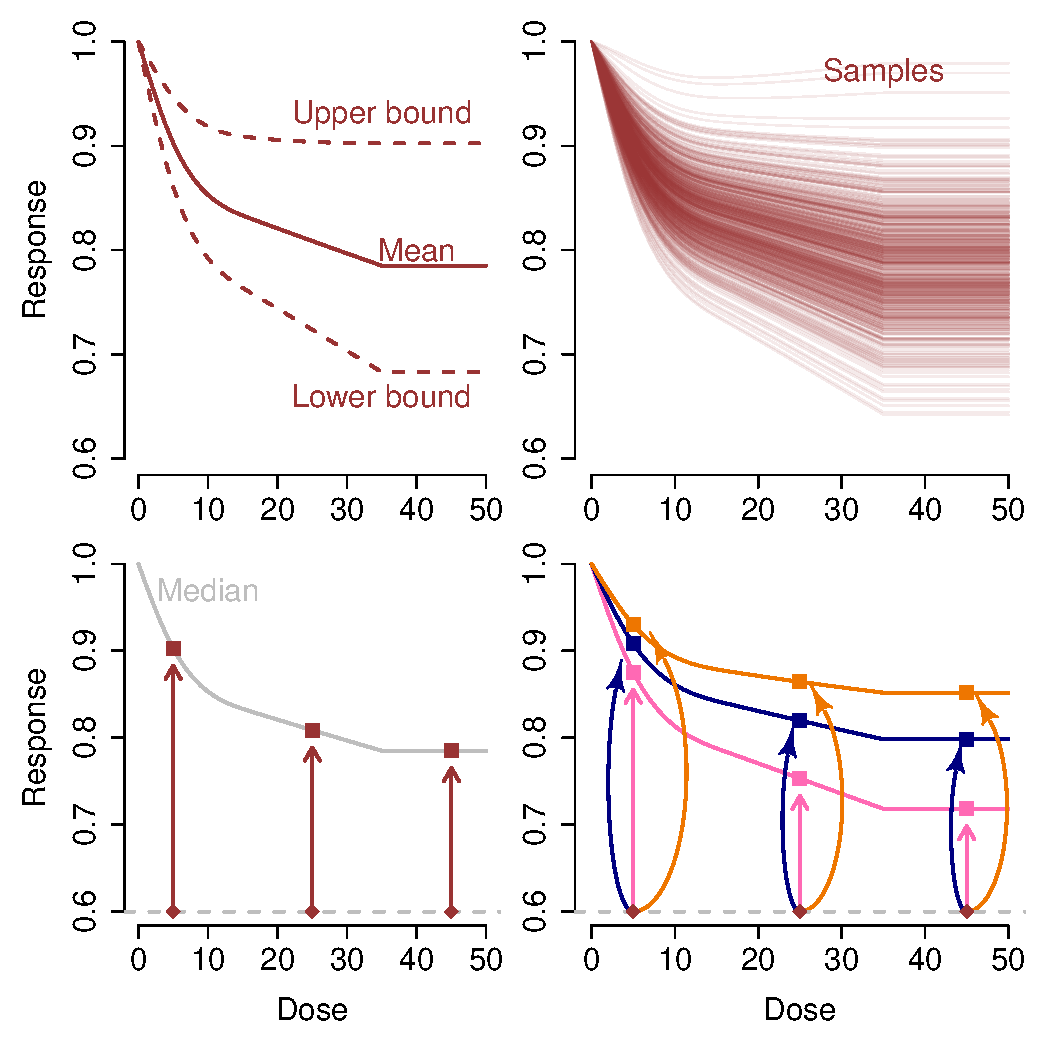
\includegraphics[width=0.6\textwidth]{cancer_PA_dose_response.pdf}
\caption{\small Example of the dose--response workflow for PA and total cancer. Top left: results of the metaanalysis: mean, lower bound and upper bound of the relationship between PA dose and relative risk of disease. Top right: examples of 500 samples from the normal distribution defined by the mean of the top-left panel and the standard deviation defined by (upper bound minus lower bound) divided by 1.96 and truncated at 0. Bottom left: relative risks of individuals with PA doses 5, 25 and 45 are found by mapping their doses onto the median curve. This is used in the ``constant'' ITHIM use case. Bottom right: relative risks of individuals with PA doses 5, 25 and 45 for three different samples from the distribution shown in the top-right panel. For each sample, each individual is mapped onto the response curve it defines. }
\label{cancer}
\end{figure}
  
\subsection{Injury module}

\subsubsection{Processing}

For the injury module, we require distance per travel mode per demographic group per scenario. It requires matching of mode names in the travel survey to mode names in the injury records, for example ``taxi'', ``shared auto'', ``shared taxi'' and ``car'' combine to form ``car''. Some work is required to separate drivers from passengers; we currently assume all travellers are drivers, with the exception of ``bus''.\footnote{This is a problem for the examples of Delhi and Bangalore, whose trip sets have car travellers under the age at which driving is permitted and who therefore should not contribute to striking distance.}

\subsubsection{Modelling}

We model injuries via regression by predicting the number of fatalities of each demographic group on each mode, which we calculate as a sum over all the ways in which they might have been injured (i.e., all the modes with which they might have collided). 

The predictive covariates include the distances travelled by the parties and their demographic details. These requirements lead to a natural separation of the (training) dataset into two groups: a set for which we have distance data for the other party, and a set for which we do not have distance data for the other party. The former equates to a ``who hit whom'' (``whw'') matrix (albeit in a higher dimension), and will account for changes in injuries resulting of a change in strike-mode travel. The latter corresponds to causes of injury that will not change across scenarios, including ``no other vehicle'' and modes of transport that we do not consider to change, which might include trucks and buses if they are not somehow explicitly included in the trip set. We label this group ``noov'': no or other vehicle.

We model the number of injuries as a Poisson-distributed variable with an offset depending on the distance(s) and the reporting rate. We write the model as follows:
\begin{align}
\tilde{I}_{a,g,m_{\text{cas}},m_{\text{str}},s,y} \sim &
\text{Poisson}(\bar{I}_{a,g,m_{\text{cas}},m_{\text{str}},s}); \\
% 'count~
\log\left(\bar{I}_{a,g,m_{\text{cas}},m_{\text{str}},s}|m_{\text{str}}\in\{m_{\text{whw}}\}\right) = &
% cas_mode*strike_mode-log(injury_reporting_rate)+log(weight)
{\kappa_0} +\sum_{i=1}^n\kappa_iX_i-\log(\sigma)+\nonumber\\
% +log(cas_distance)
 & \log(\bar{T}_{a,g,m_{\text{cas}},s})
 % +(CAS_EXPONENT-1)*log(cas_distance_sum)
 +(E_{m_{\text{cas}}}-1)\log(\hat{T}_{m_{\text{cas}},s})
 %+log(strike_distance)+(STR_EXPONENT-1)*log(strike_distance_sum)
 +E_{m_{\text{str}}}\log(\hat{T}_{m_{\text{str}},s});\\
\log\left(\bar{I}_{a,g,m_{\text{cas}},m_{\text{str}},s}|m_{\text{str}}\in\{m_{\text{noov}}\}\right) =&
{\kappa'_0}
+\sum_{i=1}^n\kappa'_iX'_i 
-\log(\sigma)
% +log(cas_distance)
+ \log(\bar{T}_{a,g,m_{\text{cas}},s})
 % +(CAS_EXPONENT-1)*log(cas_distance_sum)
 +(E_{m_{\text{cas}}}-1)\log(\hat{T}_{m_{\text{cas}},s}).
\end{align}
We choose this form of equation to enable (a) linearity in injuries with respect to total travel combined across modes and (b) linearity in injuries as subdivided by travellers of each mode.\footnote{Note that the assymmetry in the offset term for the whw expression arises due to the absence of demographic information for striking vehicles. Were we to have that, the offset would read $\log(\bar{T}_{a,g,m_{\text{cas}},s})+(E_{m_{\text{cas}}}-1)\log(\hat{T}_{m_{\text{cas}},s})+\log(\bar{T}_{a,g,m_{\text{str}},s})+(E_{m_{\text{str}}}-1)\log(\hat{T}_{m_{\text{str}},s})$. For our case, the latter two terms simplify to $\log(\hat{T}_{m_{\text{str}},s})+(E_{m_{\text{str}}}-1)\log(\hat{T}_{m_{\text{str}},s})=E_{m_{\text{str}}}\log(\hat{T}_{m_{\text{str}},s})$.} Note that this methodology is under development. See \url{https://github.com/robj411/safety_in_numbers_power_law}.

In general, one makes the best model that one can with the data available. We use, for Accra, the covariates \texttt{casualty mode*strike mode, casualty age,} and \texttt{casualty gender}, to form the model matrix $X$. We also have another covariate, \texttt{year}, but our travel data are for one year only, so we model instead many observations of the same quantities. 

We fit the coefficients $\kappa$ of the model using data for ten years, assuming the same travel each year, which corresponds to the scenario $s=\text{baseline}$. To incorporate the injury reporting rate ($\sigma$), we set it as an offset, whose value is 1 in fitting the model, and as specified in making predictions. %(For settings where there are no demographic data, we fit the model using \texttt{casualty mode} and \texttt{strike mode} alone. Predictions are made, as before, by demographic group. )

\subsubsection{Prediction}

We predict the number of injuries in each scenario based on the training model built from the baseline scenario. For Accra, we predict for the year 2016, using scenario-specific travel data.
The number of fatalities is taken as the sum of fatalities over the strike modes:
$$\check{I}_{a,g,m,o=\text{death},s}=\sum_{m_{\text{str}}}\tilde{I}_{a,g,m_{\text{cas}},m_{\text{str}},s}.$$
We extrapolate injury deaths to injury YLLs via the ratio in the GBD:
$$R_{a,g}=U_{a,g,h=\text{road injuries},o=\text{YLL}}/U_{a,g,h=\text{road injuries},o=\text{death}},$$
$$\check{I}_{a,g,m,o=\text{YLL},s}=\check{I}_{a,g,m,o=\text{death},s}\cdot R_{a,g}. $$
  
\subsection{Health module}
\subsubsection{PA and AP relative risks combined}

  We combine the relative risks of disease as a function of AP and disease as a function of PA through multiplication:
  $$\tilde{W}_{h,i,s}=W_{h,i,s}\cdot\check{H}_{h,i,s}. $$
  Not all diseases have a dose--response relationship for both AP and PA. Just stroke, lung cancer, and IHD have both. For the other diseases, only one of $W_{h,i,s}$ and $\check{H}_{h,i,s}$ is different from one.
  
  \subsubsection{Total disease burden}

We calculate the total health burden relative to the reference scenario (which, for our Accra example, is the baseline) using the injury and health outputs combined with GBD data, via population attributable fractions (PAF). The PAF is defined:
$$\hat{W}_{a,g,h,s}=\smashoperator{\sum_{\substack{i:a(i)=a,\\g(i)=g}}}\tilde{W}_{h,i,s}.$$

We then calculate the PAF relative to the reference scenario (``ref'') as:
$$\bar{W}_{a,g,h,s}= \frac{\hat{W}_{a,g,h,s=\text{ref}}-\hat{W}_{a,g,h,s}}{\hat{W}_{a,g,h,s=\text{ref}}}.$$

We estimate the background burden of disease using GBD data and scaling based on the ratio of populations between country and city. For country populations $N_{a,g}$, city populations $\bar{N}_{a,g}$ and country burden $U_{a,g,h,o}$, we estimate city burden as
$$\bar{U}_{a,g,h,o}=U_{a,g,h,o}\frac{\bar{N}_{a,g}}{N_{a,g}}.$$

If we are scaling the background burden of non-communicable diseases (``Neoplasms'', ``Ischemic heart disease'', ``Tracheal, bronchus, and lung cancer'', ``Breast cancer'', ``Colon and rectum cancer'', ``Uterine cancer''), we do so here. (Otherwise set $\rho\equiv 1$.)
$$\tilde{U}_{a,g,h,o}=\rho_h\cdot  \bar{U}_{a,g,h,o}.$$

We combine the burden with the PAF:
$$\hat{U}_{a,g,h,o,s}=\bar{W}_{a,g,h,s}\cdot\tilde{U}_{a,g,h,o}.$$

\subsubsection{Injury burden}

And, finally, for the injuries, we sum over modes to compute the burden,
$$\bar{U}_{a,g,o,s}=\sum_m\check{I}_{a,g,m,o,s},$$
and subtract from the values for the reference scenario:
$$\hat{U}_{a,g,h=\text{road injury},o,s}=\bar{U}_{a,g,o,s=\text{ref}}-\bar{U}_{a,g,o,s}.$$





\section{Example: Accra}\label{example}

Here we show the ITHIM as evaluated for the city of Accra, with a simple scenario of every person in the synthetic population gaining a single, 1 km walk. We define XX uncertain univariate parameters (Section \ref{uni}), two confidences, and two uncertain parameter sets (Section \ref{dr}). 

\subsection{Parametric distributions for uncertain variables}\label{uni}

The XX uncertain univariate parameters are shown in Figure \ref{distributions}. Most of the parameters are self explanatory. Cycling and walking MMETs are the number of MMETs per hour when undertaking cycling and walking, and determine also the ventilation rates. Motorcycle distance is the total distance travelled by motorcycles relative to the total distance travelled by cars in the baseline scenario.  Non-travel PA, injury reporting rate and NCD burden all act as scalars for the corresponding datasets. Note that the non-travel PA scalar does not affect the $\approx$40\% of the population whose non-travel PA is 0. 

\begin{figure}[h]
\centering
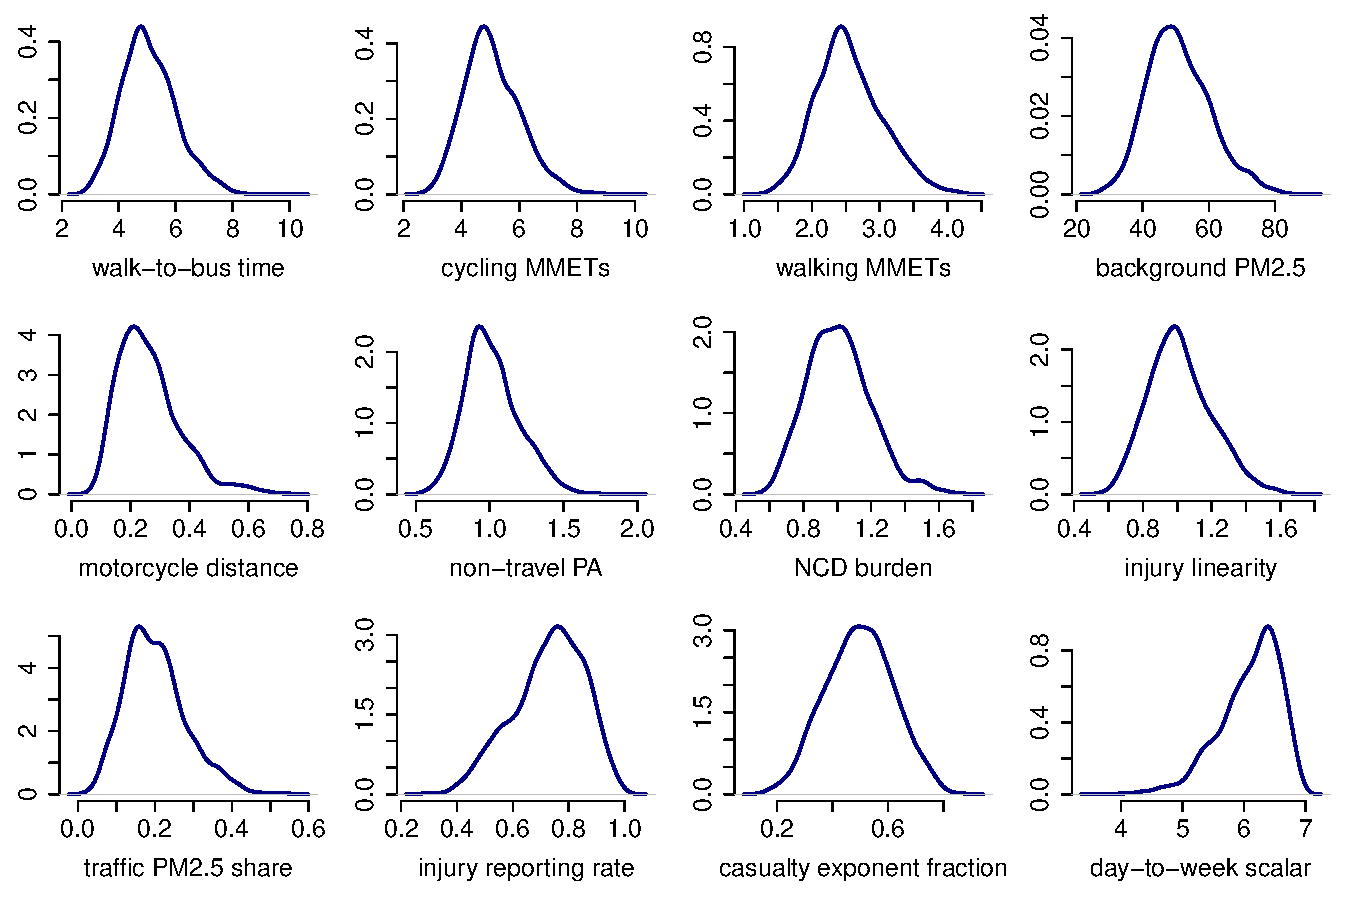
\includegraphics[width=0.95\textwidth]{uncertain_parameters.pdf}
\caption{\small Distributions of univariate uncertain parameters (1024 samples).}
\label{distributions}
\end{figure}

\subsection{Confidences}

For physical activity propensity and emission inventories, we use ``confidences'', values between 0 and 1 that represent how confident we are about the data source. We map these values to Beta (Figure \ref{prob_zero_PA}) and Dirichlet (Figure \ref{emission_dist}) distributions, respectively. The Beta-distributed propensity towards non-travel physical activity is described in Section \ref{beta}. The Dirichlet-distributed emissions inventory is described in Section \ref{dir}.


\begin{figure}[h]
\centering
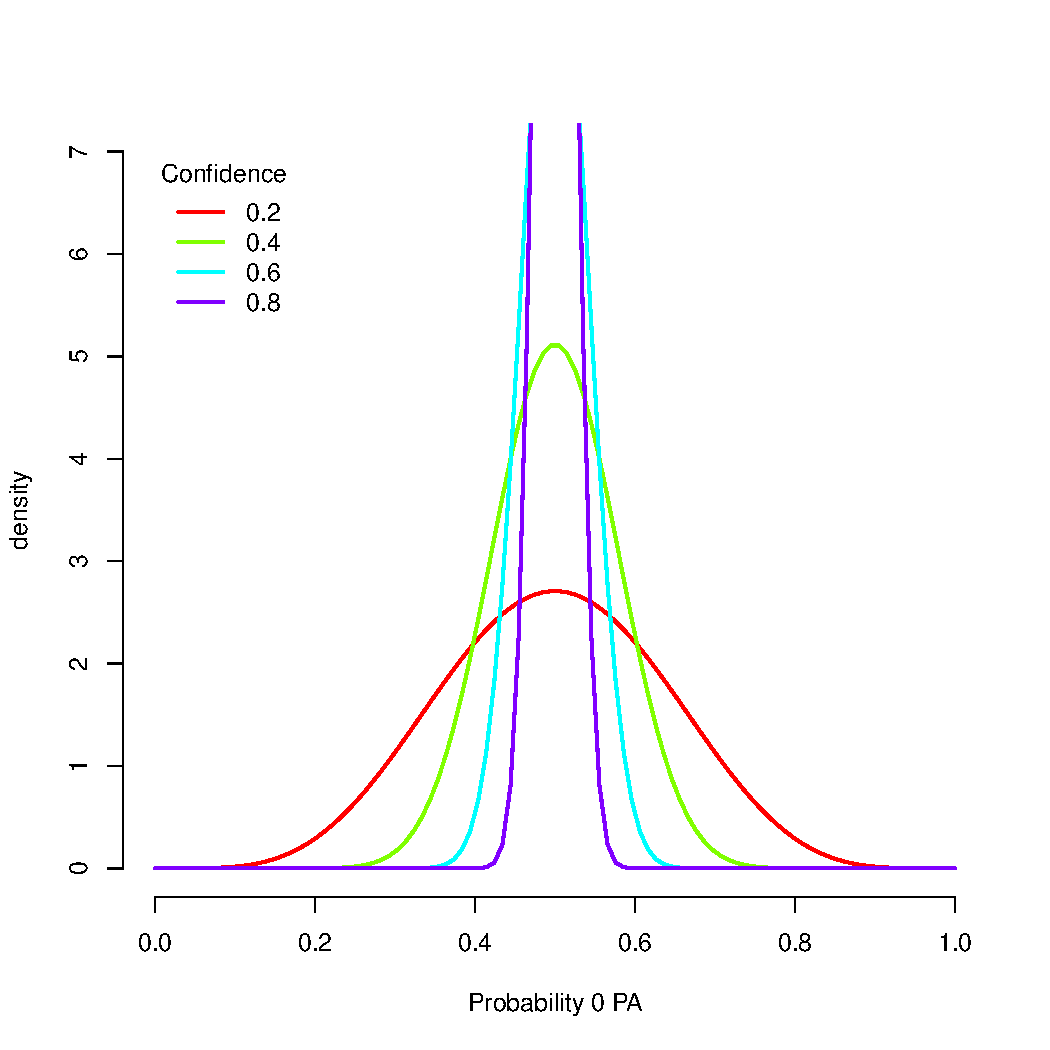
\includegraphics[width=0.5\textwidth]{prob_zero_PA.pdf}
\caption{\small Distributions of a Beta-distributed propensity to non-travel PA with varying confidence values in the raw input data. The sampled value gives the fraction of the population that engages in non-travel PA. \hl{[Re-do with Accra parameters.]}}
\label{prob_zero_PA}
\end{figure}

\begin{figure}[h]
\centering
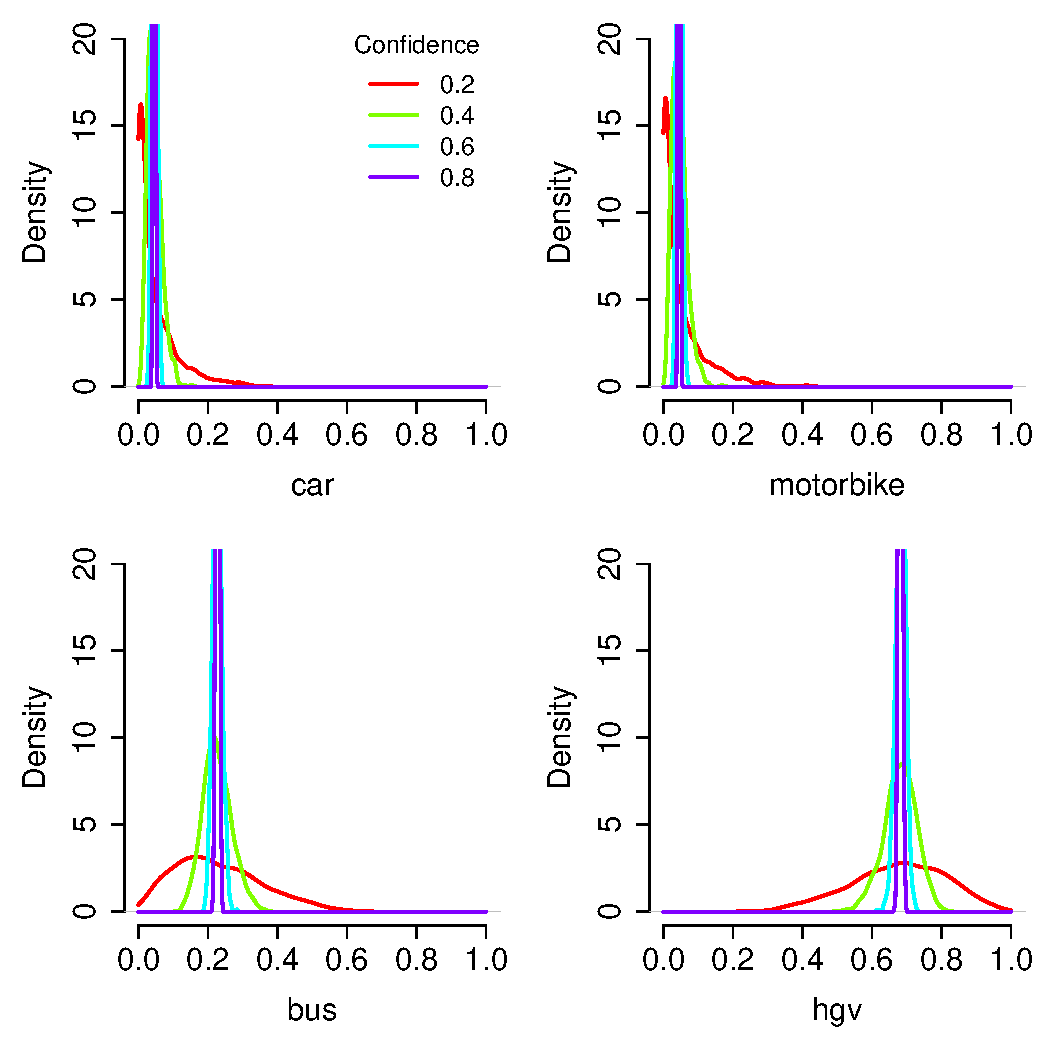
\includegraphics[width=0.65\textwidth]{emission_dist.pdf}
\caption{\small Distributions of Dirichlet-distributed emission inventories for four modes and varying confidence values. Raw input values were 4, 4, 20, and 60. \hl{[Re-do with Accra parameters and inventory.]}}
\label{emission_dist}
\end{figure}

\subsection{Dose--response relationships}\label{dr}

For the dose--response relationships between physical activity (PA) and disease and air pollution (AP) and disease, we assume that there is uncertainty, but no variability, in the relationship. This means that we sample a relationship from the distribution of relationships, and apply that relationship to all individuals precisely. This means that, given fixed doses, responses between individuals will be perfectly correlated.

We achieve this by use of the probability integral transform: we sample a random variable uniformly distributed on the space (0,1) and map it, via a cumulative distribution function, to the distribution describing the dose--response relationship. See Figure \ref{cdf} for an illustration.

\begin{figure}[h]
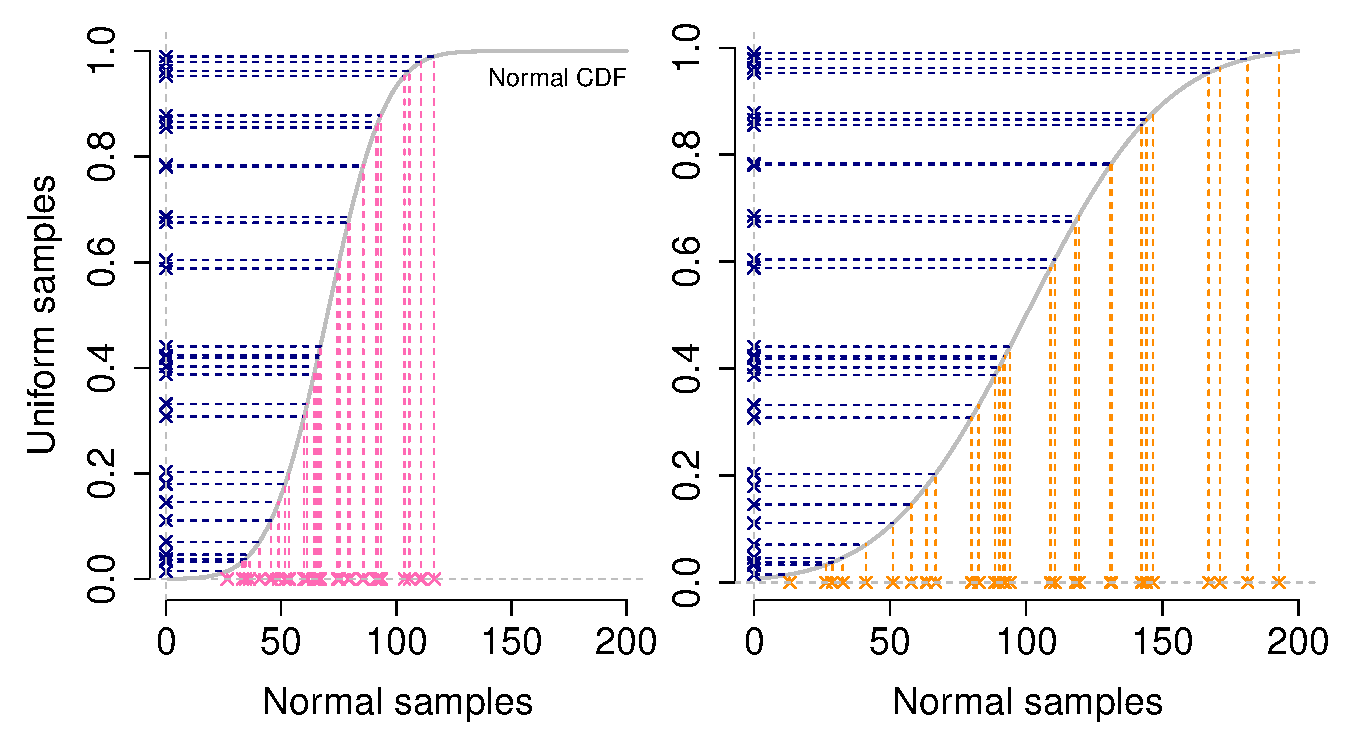
\includegraphics[width=0.8\textwidth]{DR_transform.pdf}
\caption{\small We use the same uniform samples to generate random variables from different distributions. It means that the samples are perfectly correlated.}
\label{cdf}
\end{figure}

\subsubsection{Physical activity}

Each disease's PA dose--response relationship is defined by a truncated normal. For each dose, there is a mean value, an upper bound, and a lower bound. For each person's dose, we get the response by mapping the uniform random variable onto the truncated normal defined by the mean and bounds for that dosage.

\subsubsection{Air pollution}

For the AP relationship, there are four parameters per disease. We sample the first from an empirical distribution using the probability integral transform. We sample the second via the same method, conditioned on the value of the first, constructing their joint density with e.g. kde2d. The third parameter is sampled conditioned on the first and second, constructing their joint density using a GAM. The final parameter is sampled conditioned on the first, second, and third, constructing their joint density using a GAM.

As before, there is perfect correlation between individuals, i.e. if person A's dose is greater than person B's, then person A's response is strictly greater than person B's response.

The empirical distributions come from \citet{Burnett2014}. There are four parameters per disease: IHD, lung cancer, COPD, stroke, and LRI. In addition, for stroke and IHD, there is a set of four parameters for each age group from 25 to 95 in five-year increments. In addition to our assumption that there is perfect correlation between individuals for diseases, we assume perfect correlation between ages for diseases. I.e., our four quantiles per disease will be applied to all age groups. 
\clearpage
\section{Results}\label{results}
\subsection{Health burdens in scenarios}
%The scenarios for Accra are:
%\begin{itemize}
%\item Baseline (base) -- the current state of affairs
%\item Scenario 1 (scen1) --  bus + walk to car 
%\item Scenario 2 (scen2) -- scen1 plus long trips from car + taxi to bus 
%\item Scenario 3 (scen3) -- scen1 plus car to motorbike 
%\item Scenario 4 (scen4) -- scen1 plus short trips from car + taxi + motorbike to cycle 
%\item Scenario 5 (scen5) -- scen1 plus short trips from car + taxi to walk
%\end{itemize}

\begin{comment}
\begin{figure}[h]
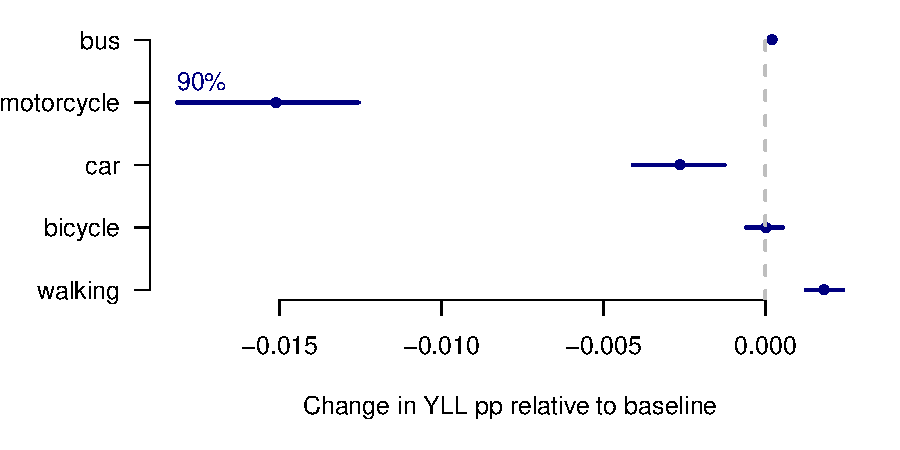
\includegraphics[width=0.8\textwidth]{combined_yll_pp.pdf}
\caption{\small Results (YLLs per person) for four cities combined, relative to scen1.}
\label{results}
\end{figure}

\begin{figure}[h]
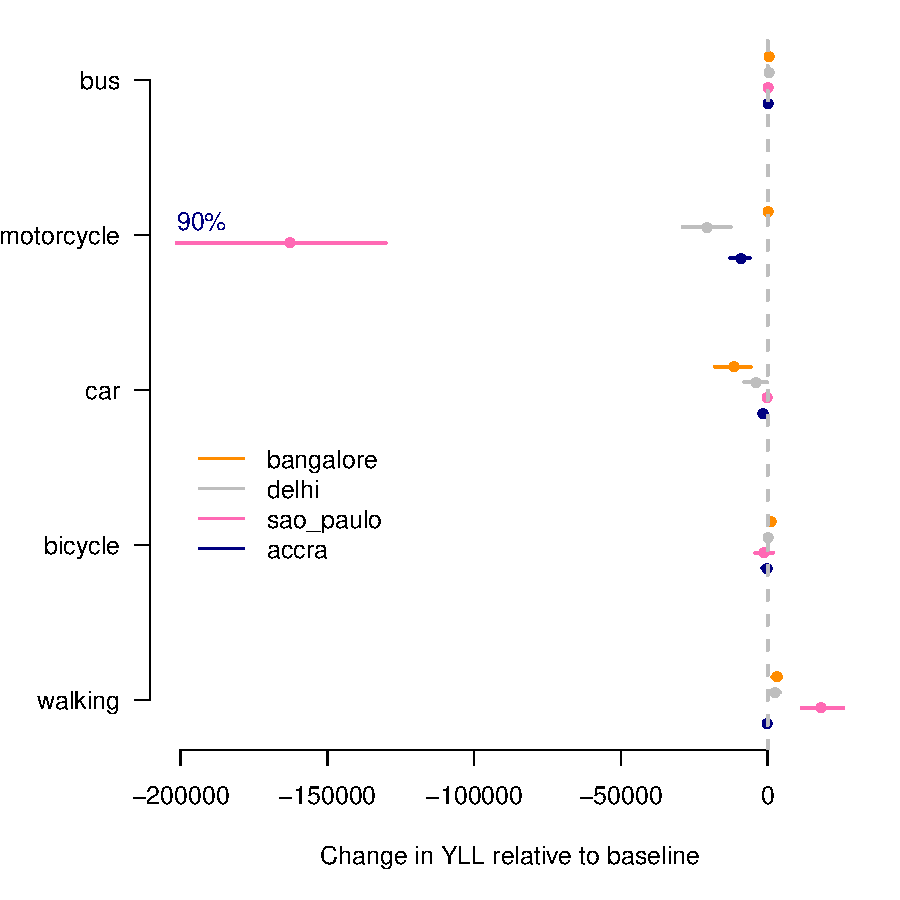
\includegraphics[width=0.8\textwidth]{city_yll.pdf}
\caption{\small Results (YLLs) for four cities, relative to scen1.}
\label{results}
\end{figure}
\end{comment}

\begin{figure}[h]
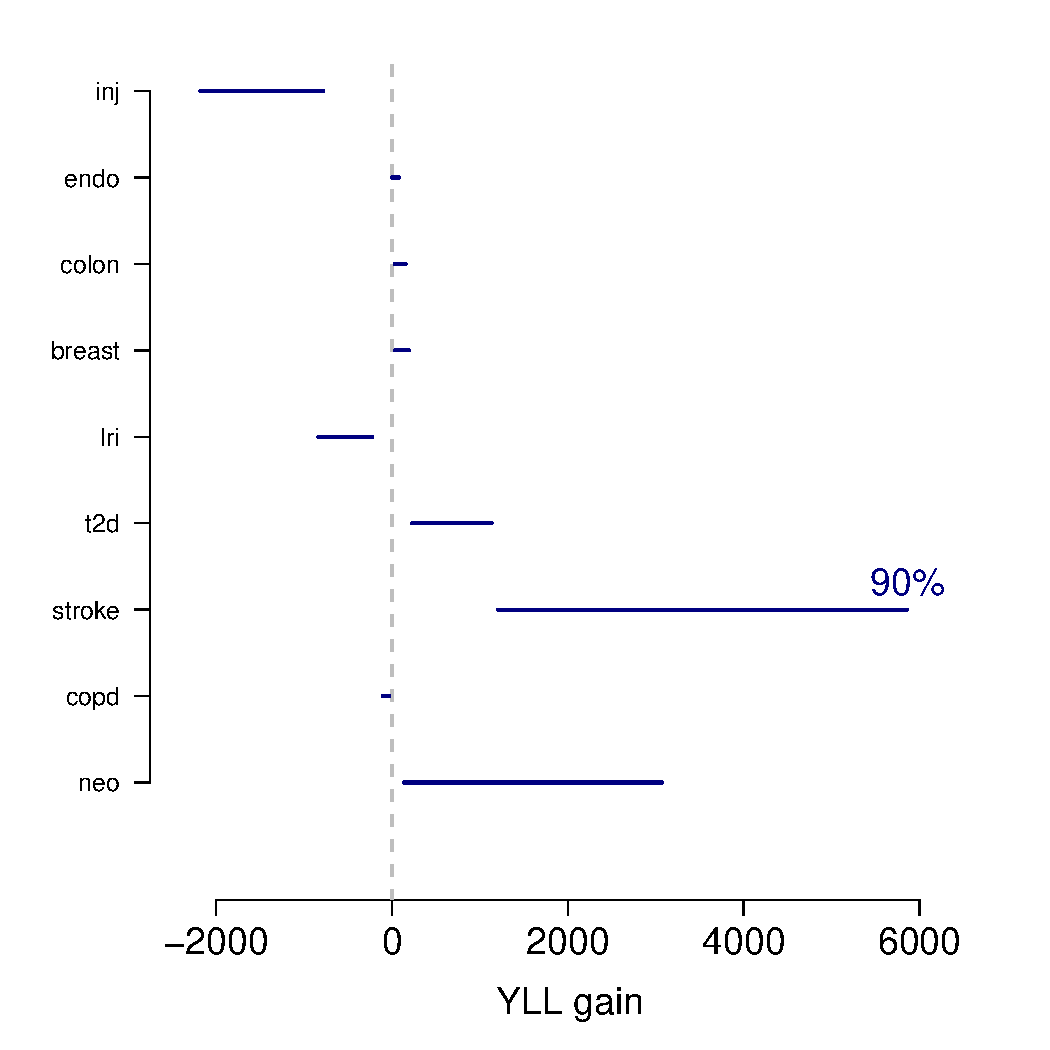
\includegraphics[width=0.8\textwidth]{accra_walk_yll.pdf}
\caption{\small YLLs in the scenario minus YLLs in the baseline for Accra.}
\label{results}
\end{figure}
\clearpage
\subsection{Value of information}

We calculate value of information following \citet{Jackson2017}. The ``value of information'' we implement is the expected value of perfect partial information (EVPPI). It is the expected amount by which variation in the outcome diminishes should a parameter, or set of parameters, be known perfectly. With reference to information theory, it is the mutual information between the parameter, or parameter set, and the outcome, where the outcome is described only by its second moment (its variance). 

The objective of learning the value of information formulated in this way is to identify the parameter or parameters that most drive variability (variance) in the outcome. The results guide future research, identifying which area or areas offer the greatest benefit in terms of prediction accuracy given further research. For example, for our model of Accra, learning better the dose--response relationship between physical activity and stroke (incidence) would likely increase precision of our estimate of total years of life lost (YLL) more so than learning any other parameter (Figure \ref{evppi}).

\begin{figure}[h]
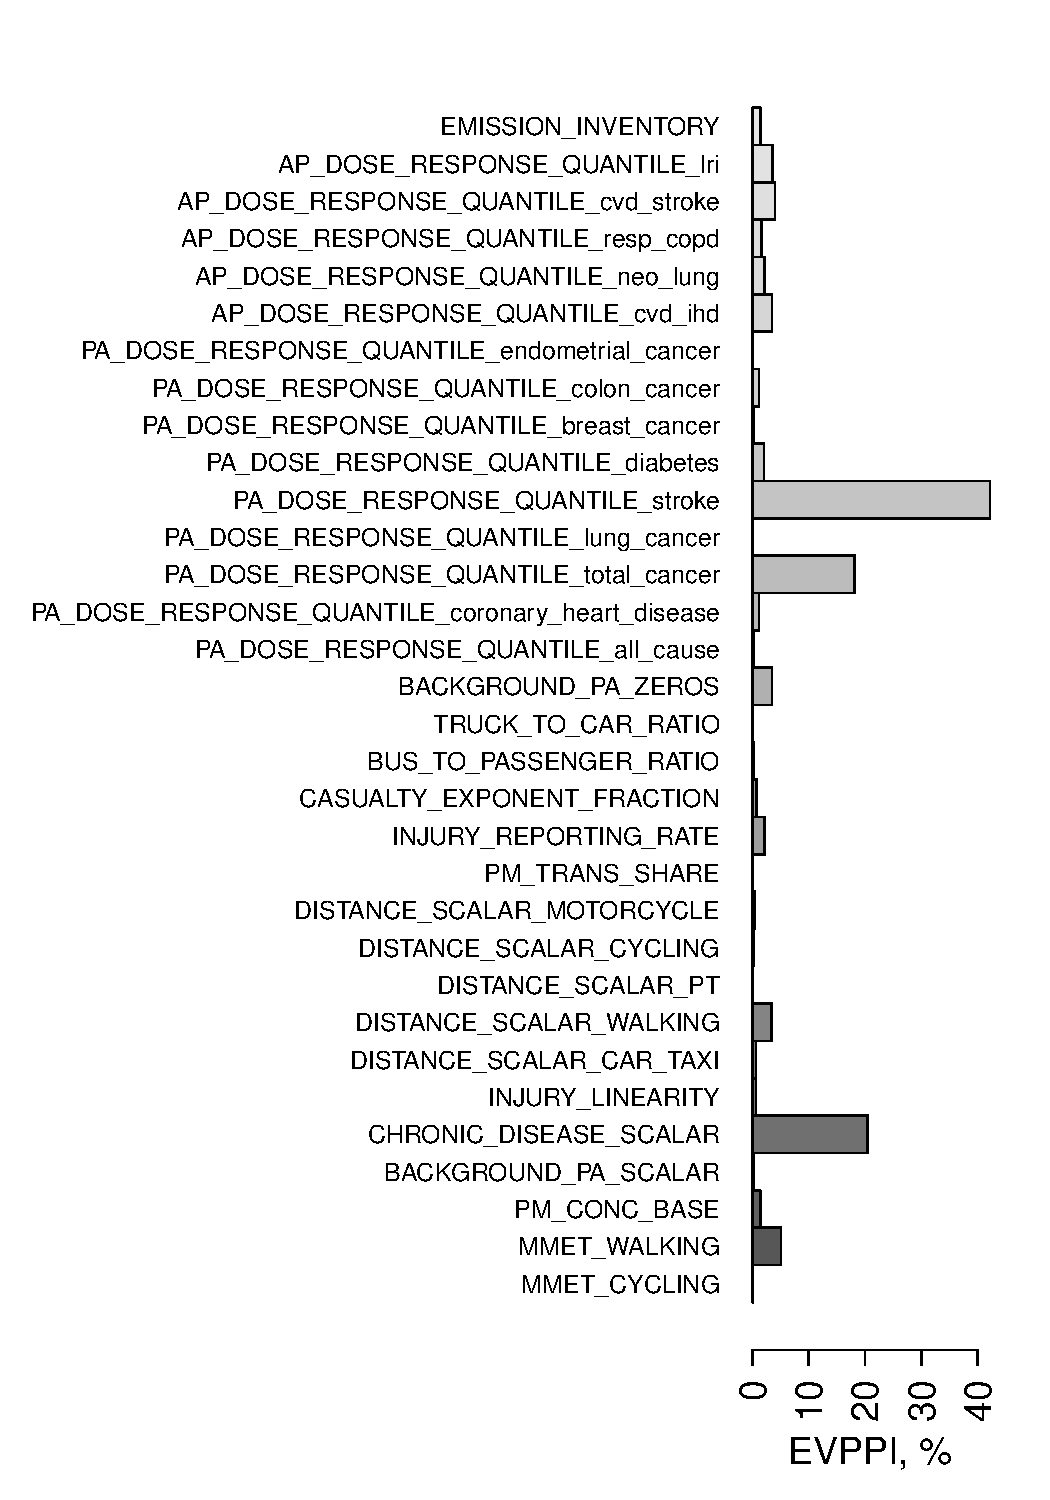
\includegraphics[width=0.7\textwidth]{accra_walk_evppi.pdf}
\caption{\small EVPPI for Accra's ``walking'' scenario for all causes of YLLs excluding ``all cause'' and ``neoplasm''.}
\label{evppi}
\end{figure}
\clearpage


\begin{appendix}

\section{ITHIM with parameters}

\begin{figure}[h]
  \centering
  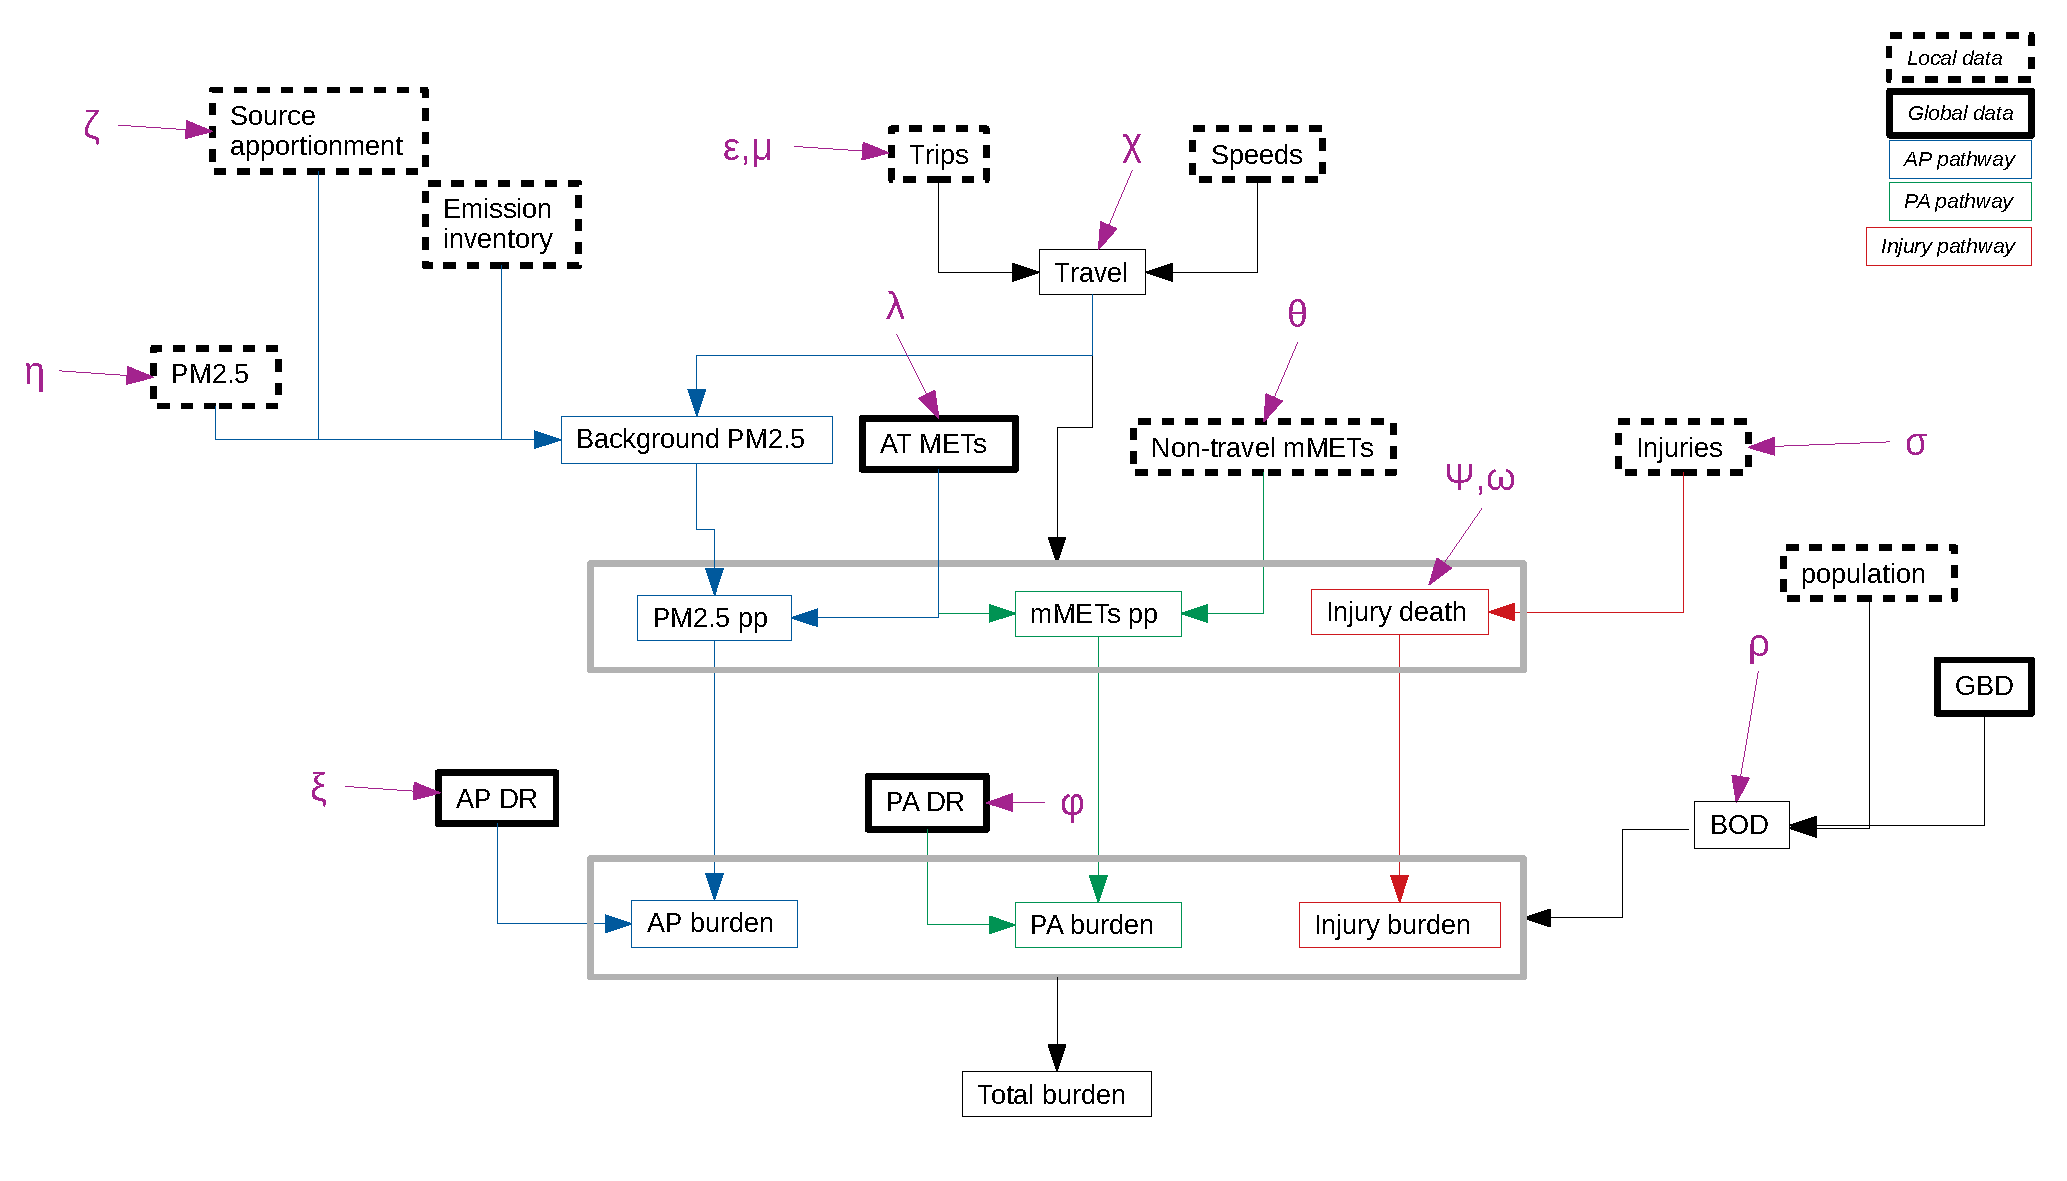
\includegraphics[width=\textwidth]{ithim_with_parameters.pdf}
  \caption{\small ITHIM-R workflow, with variable parameters in purple. Fixed inputs to the model have a bold, black outline, which is solid for inputs we consider ``global'' and dashed for inputs we consider ``local''. There are four global inputs, which will be embedded in ITHIM-R. There are seven local inputs, which users should provide. The graph depicts parent--child relationships, where a child (at the head of an arrow) depends upon all its parents (at the source(s) of the arrow(s)). To aid visualisation, an arrow connected to the outside of a grey box indicates that the arrow connects to each item within the box. \textit{AT: active travel. MET: metabolic equivalent task. pp: per person. AP: air pollution. PA: physical activity. DR: dose--response relationship. GBD: global burden of disease.} NB: $\rho$ only impacts the NCD burden of GBD, not all of it. Missing parameter: motorcycle distance. $\lambda$ is a 2D parameter. $\xi$ is 4D.}
\label{ithim_with_parameters}
\end{figure}

\clearpage
\section{Dose--response relationships}

\begin{figure}[H]
\centering
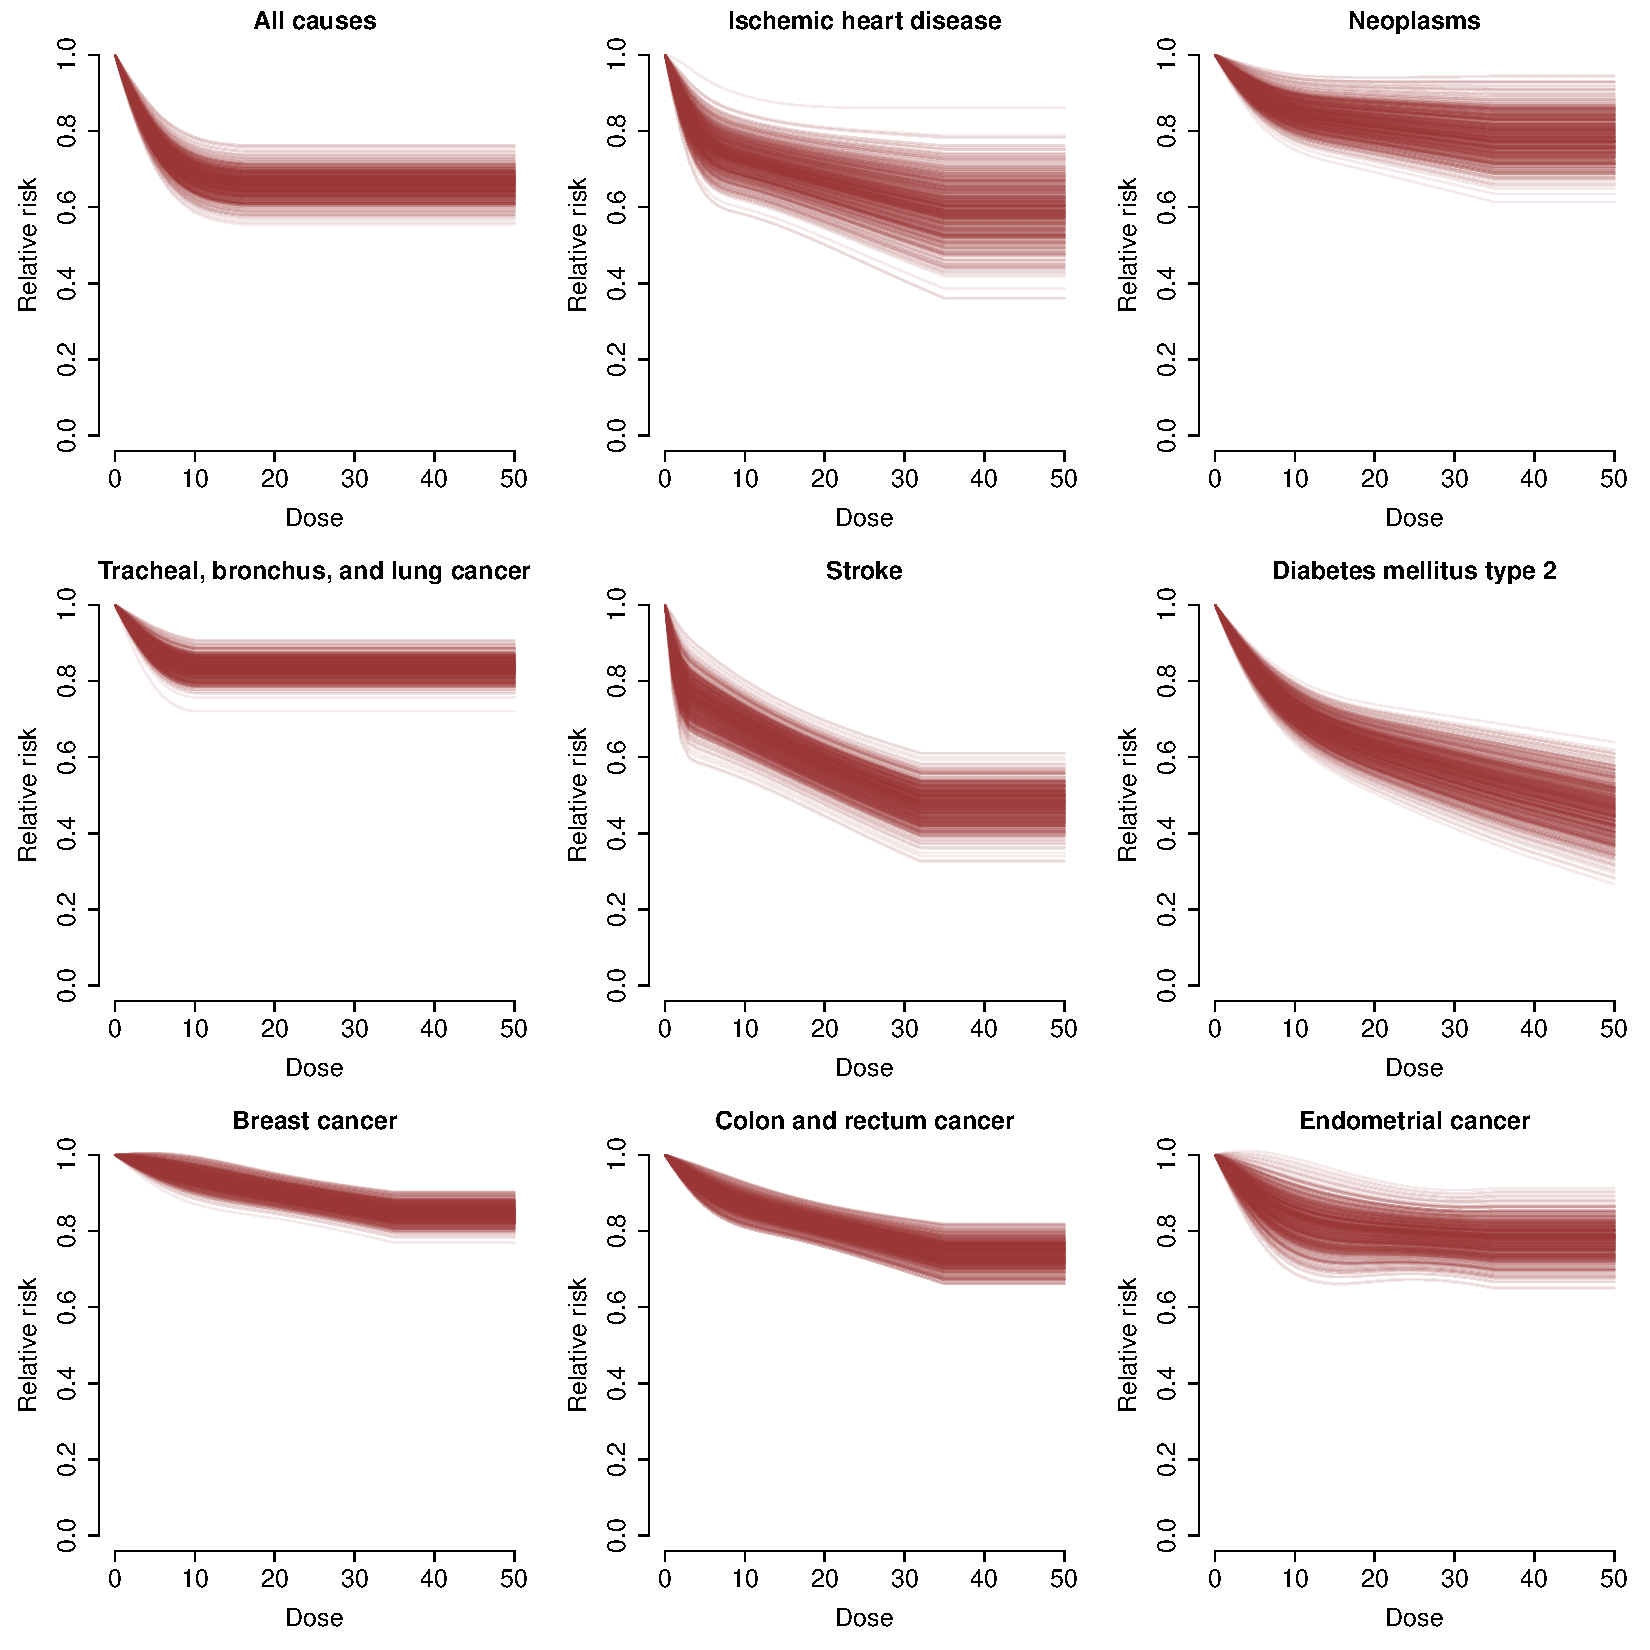
\includegraphics[width=0.9\textwidth]{PA_dose_response.pdf}
\caption{\small 1000 samples from PA dose--response curves}
\label{PADR}
\end{figure}

\begin{figure}[H]
\centering
\begin{tabular}{cc}
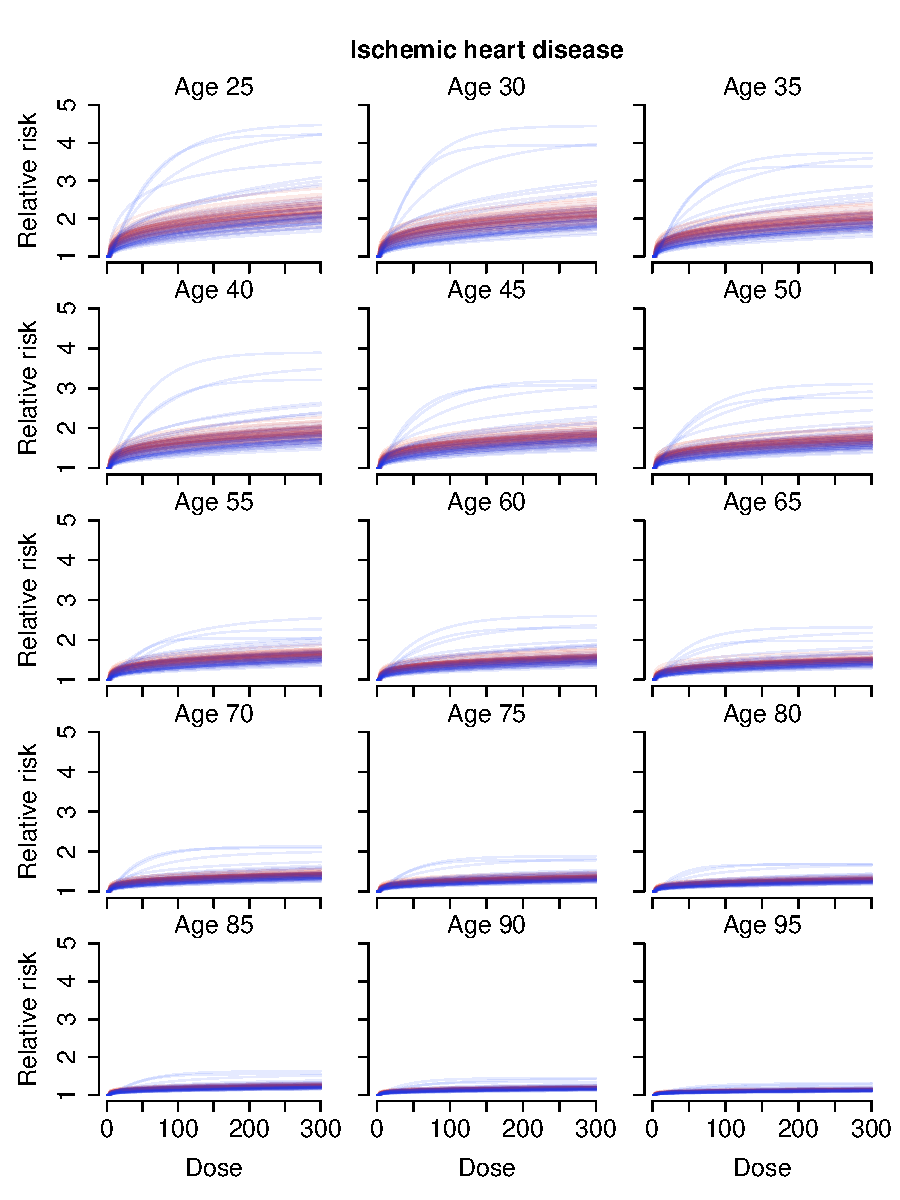
\includegraphics[width=0.4\textwidth]{cvd_ihdDR-sim.pdf}&
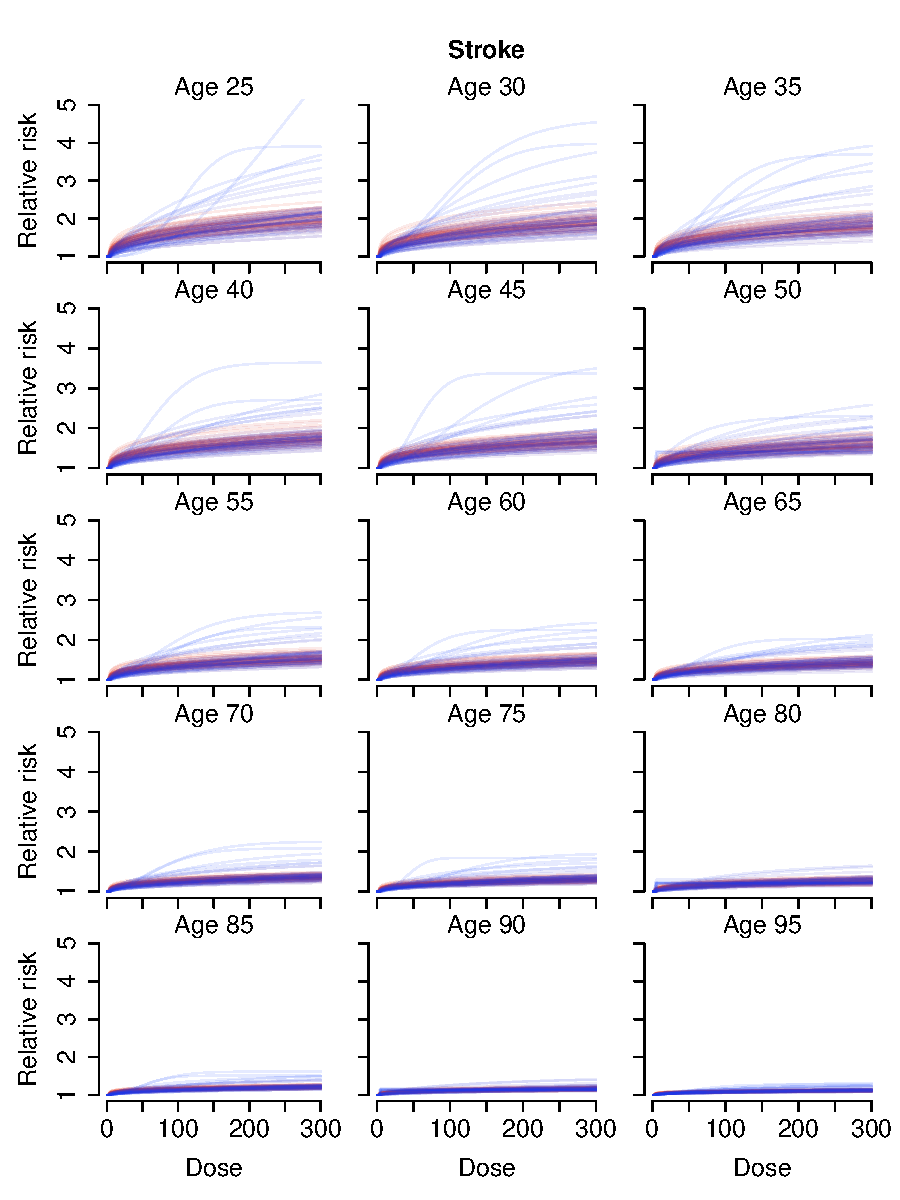
\includegraphics[width=0.4\textwidth]{cvd_strokeDR-sim.pdf}\\
\end{tabular}
\begin{tabular}{ccc}
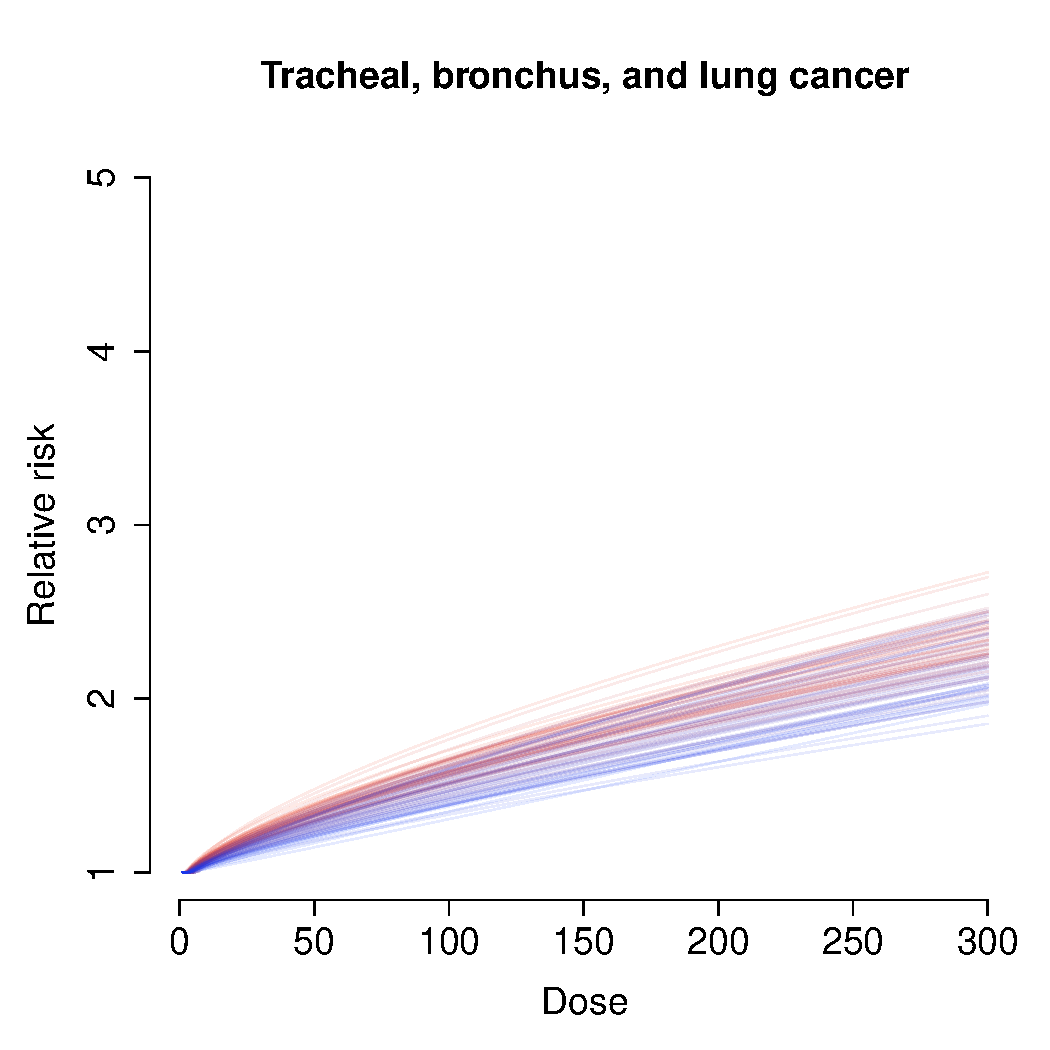
\includegraphics[width=0.3\textwidth]{neo_lungDR-sim.pdf}&
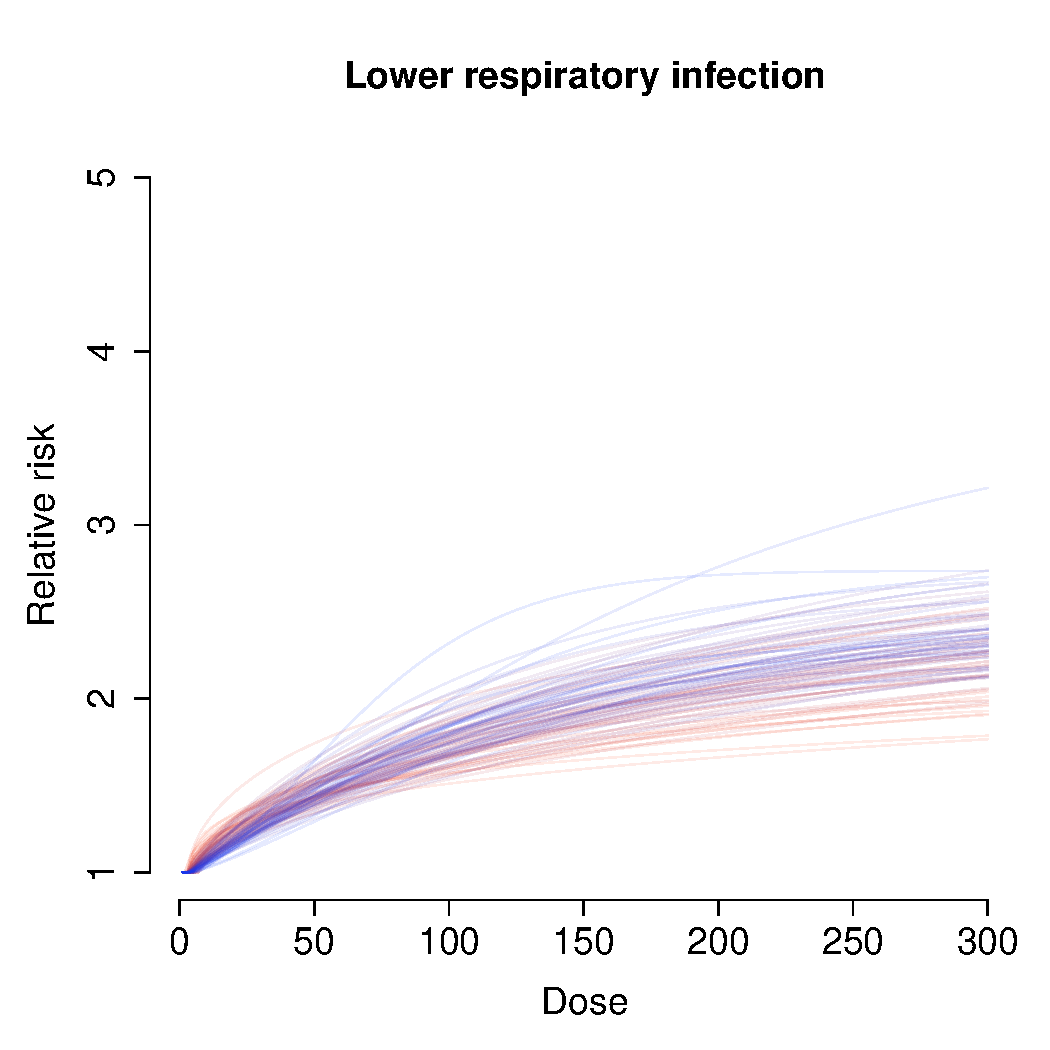
\includegraphics[width=0.3\textwidth]{lriDR-sim.pdf}&
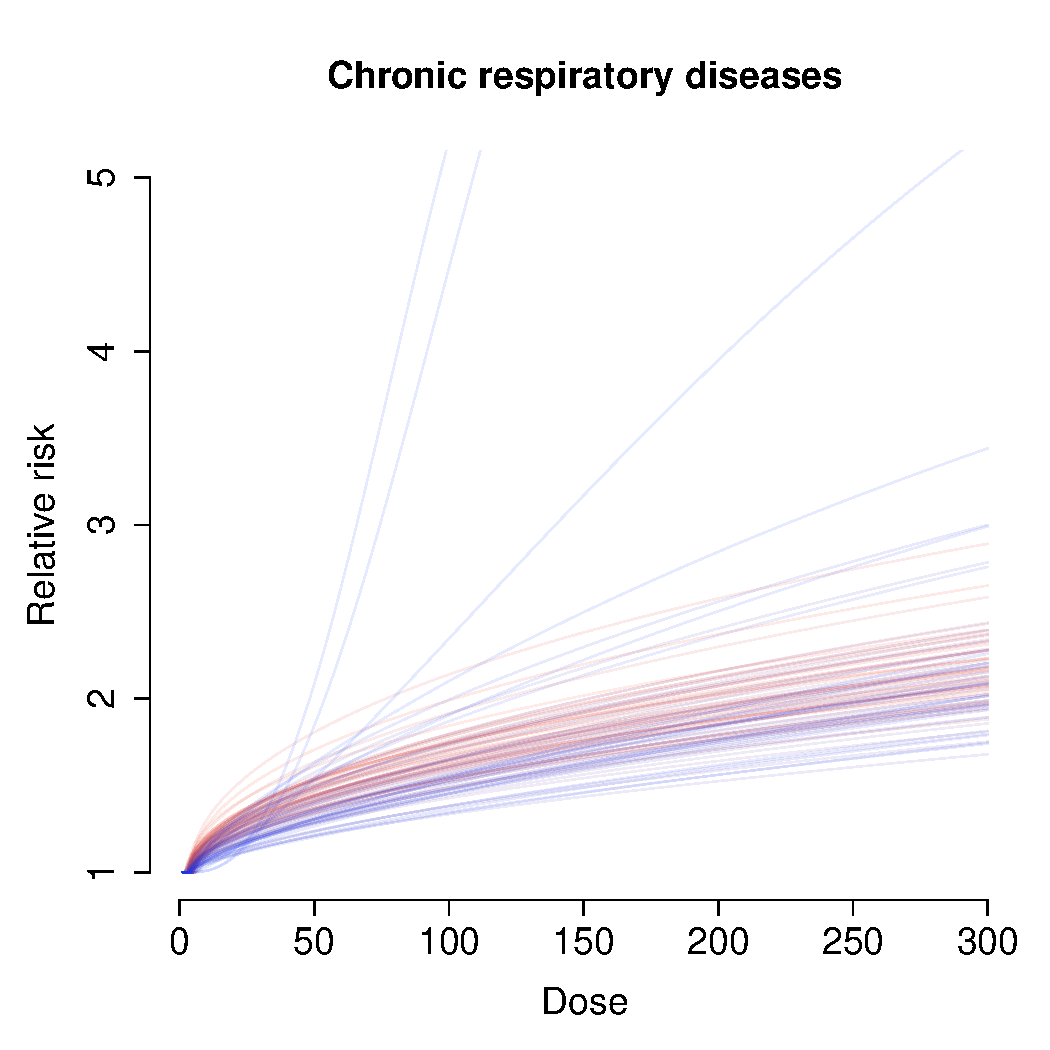
\includegraphics[width=0.3\textwidth]{resp_copdDR-sim.pdf}\\
\end{tabular}
\caption{\small 100 samples from AP dose--response curves}
\label{APDR}
\end{figure}




\clearpage

\begin{landscape}
\section{Tabulated ITHIM equations}\label{tableequations}

\begin{center}
\begin{ThreePartTable}
  \begin{TableNotes}  
  \small
  \item[\textdagger] {\footnotesize CDF: cumulative distribution function. We use generative distributions to generate random numbers so that samples are correlated. For $t=\text{CDF}_{F}^{-1}(q)$, $t$ is the $q$-th quantile of function $F$ with CDF CDF$_F$. (I'd like to find an improved notation for this.)}
  \end{TableNotes}
\begin{longtable}{lp{7cm}p{5cm}}
\caption{\small All calculations in the ITHIM.}\label{calculationstab}\\
Name & Description & Label \\
\hline
\multicolumn{3}{l}{\textit{Scenario generation}}\\
\hline
...&&\\[5pt]
\hline
\multicolumn{3}{l}{\textit{Travel calculations}}\\
\hline
$\{T_{j^+}\leftarrow \epsilon; m(j^+)\leftarrow\text{walk}\}\, \forall\, T_j:m(j)=\text{bus}$ &New walk trips to bus&{walk\_to\_bus\_and\_combine\_scen}\\[5pt]
%$T_j\leftarrow T_j-\epsilon\, \forall\, j:m(j)=\text{bus}\text{ \& }T_j>\epsilon$ &Subtract walk distance from bus trip&{walk\_to\_bus\_and\_combine\_scen}\\[5pt]
$\bar{T}_{a,g,m,s}=\sum_{j:a(j)=a,g(j)=g,m(j)=m,s(j)=s}Q_{i(j)}T_j$ & (Weighted) total travel per age, gender, mode and scenario &  \\[5pt]
$\check{T}_{a,g,m,s}=\frac{\bar{T}_{a,g,m,s}}{\sum_{a,g}\bar{T}_{a,g,m,s}}$ & Relative travel per mode and scenario by age and gender & inj\_distances[[1]] \\[5pt]
$\hat{T}_{m,s}=\sum_{a,g}\bar{T}_{a,g,m,s}$ & Total travel per mode and scenario & dist \\[5pt]
$\tilde{T}_{m,s}=\frac{\hat{T}_{m,s}}{\hat{T}_{m,s=\text{baseline}}}$ & Total travel per mode and scenario relative to baseline, with car modes summed, and Tuktuk = 1 &  inj\_distances[[2]] \\[5pt]
\hline
\multicolumn{3}{l}{\textit{Injury calculations}}\\
\hline

$E_{m_{\text{cas}}}=\psi\omega$ & Casualty exponent & CAS\_EXPONENT  \\[5pt]

$E_{m_{\text{str}}}=\omega-E_{m_{\text{cas}}}$ & Striker exponent & STR\_EXPONENT \\[5pt]

$\tilde{I}_{a,g,m_{\text{vic}},m_{\text{str}},s}=\mathcal{S}\left(\sigma\cdot {I}_{a,g,m_{\text{vic}},m_{\text{str}}},\bar{T}_{a,g,m,s},E_{m_{\text{cas}}},E_{m_{\text{str}}}\right)$
%\cdot \tilde{T}_{m=\text{vic},s}^{S_{m_{\text{vic}},m_{\text{str}},r=\text{vic}}}\cdot \tilde{T}_{m=\text{str},s}^{S_{m_{\text{vic}},m_{\text{str}},r=\text{str}}}$
& Fatalities in scenarios by strike mode & injuries\\[5pt]
$\check{I}_{a,g,m,o=\text{death},s}=\sum_{m_{\text{str}}}\tilde{I}_{a,g,m_{\text{vic}},m_{\text{str}},s}$ & Fatalities in scenarios  & victim\_deaths\\[5pt]
%$\check{I}_{a,g,m,o=\text{death},s}=\hat{I}_{a,g,m,s}$ & Fatalities distributed to age-and-gender groups & injuries \\[5pt]

$R_{a,g}=U_{a,g,h=\text{road injuries},o=\text{YLL}}/U_{a,g,h=\text{road injuries},o=\text{death}}$ & Road YLL-to-death ratio & GBD\_INJ\_YLL\\[5pt]

$\check{I}_{a,g,m,o=\text{YLL},s}=\check{I}_{a,g,m,o=\text{death},s}\cdot R_{a,g} $ & YLLs scaled from fatalities & deaths\_yll\_injuries \\[5pt]

\hline
\multicolumn{3}{l}{\textit{Pollution calculations}}\\
\hline
$\dot{P}_{m}=\left\{\begin{array}{lr}\gamma_m & P=1 \\ \tilde{\gamma}_m, \tilde{\gamma}_m \sim \text{Dir}(f(P,\gamma_m)) & P<1 \end{array}\right.$ & Emissions by mode &   trans\_emissions \\[5pt]

$\tilde{P}_{m,s}=\dot{P}_m\hat{T}_{m,s}/\hat{T}_{m,s=\text{baseline}}$& Emissions by mode in scenario relative to baseline &   trans\_emissions \\[5pt]

$\hat{P}_{s}=\sum_{m} \tilde{P}_{m,s}$ & Emissions scalar for scenarios & baseline\_sum \\[5pt]
%$\check{P}_s = \eta\zeta\hat{P}_s$ & Background PM2.5 concentration due to transport in scenarios &    \\[5pt]
$\bar{P}_s=\eta(\zeta\hat{P}_s + 1-\zeta)$ & Background PM2.5 concentration in scenarios &   scenario\_pm  \\[5pt]
\hline 
\hline 
$K_s=C_4-C_5\log(\bar{P_s})$ & On-road PM2.5 exposure ratio  & on\_road\_off\_road\_ratio \\[5pt]
$\tilde{K}_{m\in\{\text{walk,cyc.,mot.}\},s}=K_s$ & On-road PM2.5 exposure ratio for open vehicle  & on\_road\_off\_road\_ratio  \\[5pt]
$\tilde{K}_{m\in\{\text{sub.}\},s}=C_6$ & Subway PM2.5 exposure ratio   & subway\_ratio  \\[5pt]
$\tilde{K}_{m\not\in\{\text{walk,cyc.,mot.,sub.}\},s}=C_2C_3+K_s(1-C_3)$ & In-vehicle PM2.5 exposure ratio  & in\_vehicle\_ratio  \\[5pt]
\hline
\hline 
$V_m=C_1+\frac{1}{2}\lambda_m$ & Ventilation rates &   vent\_rates \\[5pt] 
$\tilde{V}_{i,m,s} = \sum_{j:i(j)=i,m(j)=m,s(j)=s}T_j\cdot V_{m(j)}/Z_{m(j)}$ & In-travel air inhaled &   \\[5pt]
$\bar{V}_{i,s} = \sum_{m}\tilde{V}_{i,m,s}\cdot \tilde{K}_{m,s}$ & In-travel PM2.5 inhalation rate &   \\[5pt]
$\hat{V}_{i,s} = C_1\left(24-\sum_{j:i(j)=i,s(j)=s}T_j/Z_{m(j)}\right)$ & Non-travel air inhaled &   \\[5pt]
$\check{W}_{i,s} = \bar{P}_s(\bar{V}_{i,s}+\hat{V}_{i,s})/24
%/(\sum_m\tilde{V}_{i,m,s}+\hat{V}_{i,s})
$ & Total PM2.5 inhaled per hour  &  \\[5pt]

%$\check{P}=\frac{\text{mean}(\check{V}_{i,s=\text{Baseline}})}{\bar{P}_{s=\text{Baseline}}}$ & Normalisation constant   &  \\[5pt]
%$\check{W}_{i,s} = \check{P}\check{V}_{i,s}$ & Normalised total PM2.5 inhaled   & pm\_conc\_pp \\[5pt]

\hline
\hline 
$\tilde{H}_{a,h,w=3}=\text{CDF}_{H_{a,h,w=3}}^{-1}(\xi_{h,w=3})^{\dagger}$ &{AP dose--response--curve parameter}& DR\_AP\_LIST \\[5pt]
$\tilde{H}_{a,h,w=3}=\text{CDF}_{H_{a,h,w=3}|\tilde{H}_{a,h,w=3}}^{-1}(\xi_{h,w=3})^{\dagger}$ &{AP dose--response--curve parameter}& DR\_AP\_LIST \\[5pt]
$\tilde{H}_{a,h,w=3}=\text{CDF}_{H_{a,h,w=3}|\tilde{H}_{a,h,w=3},\tilde{H}_{a,h,w=3}}^{-1}(\xi_{h,w=3})^{\dagger}$ & {AP dose--response--curve parameter} & DR\_AP\_LIST \\[5pt]
$\tilde{H}_{a,h,w=3}=\text{CDF}_{H_{a,h,w=3}|\tilde{H}_{a,h,w=3},\tilde{H}_{a,h,w=3},\tilde{H}_{a,h,w=3}}^{-1}(\xi_{h,w=3})^{\dagger}$ &{AP dose--response--curve parameter}& DR\_AP\_LIST \\[5pt]
$\check{H}_{h,i,s} = 1 + \tilde{H}_{a=a(i),h,w=3}\times$ &&\\[5pt]
$\left\{1 - \exp\left(-\tilde{H}_{a=a(i),h,w=3}  (\check{W}_{i,s} - \tilde{H}_{a=a(i),h,w=3}) ^ {\tilde{H}_{a=a(i),h,w=3} }\right)\right\}$& RR of disease given pollution &  RR\_AP\_calculations \\[5pt]


\hline 
\multicolumn{3}{l}{\textit{Physical activity calculations}}\\
\hline

$\dot{Y}_{a,g}=\text{Prob}(Y_i=0)|_{a(i)=a,g(i)=g}$ & Raw probability non-travel MMETs = 0 for demographic group $a,g$ & raw\_zero \\[5pt]

$\bar{Y}_{a,g}=\left\{\begin{array}{lr} \dot{Y}_{a,g} & \tilde{Y}=1 \\ \text{CDF}_{\text{Beta}(f(\tilde{Y},\dot{Y}_{a,g}))}^{-1}(\tilde{\theta}) & \tilde{Y}<1 \end{array}\right.$& Probability non-travel MMETs = 0 for demographic group $a,g$ &  zeros  \\[5pt]

$\check{Y}_i = \left\{\begin{array}{lr} 0 & \bar{Y}_{a(i),g(i)} \\ \text{Sample}(\{Y_{i'}\}|_{a(i')=a(i),g(i')=g(i),Y_{i'}>0}) & 1-\bar{Y}_{a(i),g(i)} \end{array}\right.$& Non-travel MMETs &  SYNTHETIC\_POPULATION\$ work\_ltpa\_marg\_met  \\[5pt]

$M_{i,s}=\sum_{j:i(j)=i,s(j)=s}(\chi T_j\cdot \lambda_{m(j)}/Z_{m(j)})+\theta \check{Y}_i$ & Total MMETs per person & mmets \\[5pt]

$\tilde{G}_{h,x}(m) = {G}_{h,x,z=\lfloor{m}\rfloor}+({G}_{h,x,z=\lceil{m}\rceil}-{G}_{h,x,z=\lfloor{m}\rfloor})\frac{m-\lfloor{m}\rfloor}{\lceil{m}\rceil-\lfloor{m}\rfloor}$ & Interpolated dose--response parameters & rr, lb, ub \\[5pt]

$F_S(s_x) = \mathcal{N}(s_{x=2},(s_{x=3}-s_{x=1})/1.96)|_{0<F_S(s_x)} $ & Truncated normal function &  \\[5pt]

$W_{h,i,s}=\text{CDF}_{F_S\left(\tilde{G}_{h,x}(M_{i,s})\right)}^{-1}\left(\phi_{h}\right)^{\dagger}$ &Relative risk of disease given PA&RR\_PA\_calculations\\[5pt]


\hline 
\multicolumn{3}{l}{\textit{Burden-of-disease calculations}}\\
\hline
$\tilde{W}_{h,i,s}=W_{h,i,s}\cdot\check{H}_{h,i,s} $ & Combined PA and AP relative risks& RR\_PA\_AP\_calculations \\[5pt]

$\hat{W}_{a,g,h,s}= \sum_{i:a(i)=a,g(i)=g}\tilde{W}_{h,i,s}$ & Population-attributable fractions& pif\_temp \\[5pt]

$\bar{W}_{a,g,h,s}= (\hat{W}_{a,g,h,s=\text{scen1}}-\hat{W}_{a,g,h,s})/\hat{W}_{a,g,h,s=\text{scen1}}$ & Population-attributable fractions relative to scenario 1& pif\_scen \\[5pt]

$\bar{U}_{a,g,h,o}=U_{a,g,h,o}\frac{\bar{N}_{a,g}}{N_{a,g}}$ & GBD scaled to local population & DISEASE\_BURDEN \\[5pt]

$\tilde{U}_{a,g,h,o}=\rho_h\cdot  \bar{U}_{a,g,h,o}$ & Scaled background disease for Neoplasms, IHD, Lung cancer& gbd\_data\_scaled \\[5pt]

$\hat{U}_{a,g,h,o,s}=\bar{W}_{a,g,h,s}\cdot\tilde{U}_{a,g,h,o}$ & Combined health and PIF & yll\_dfs, death\_dfs \\[5pt]

$\hat{U}_{a,g,h=\text{road injury},o,s}=\sum_m\check{I}_{a,g,m,o,s}$ & Injury health burden & inj \\[5pt]

\hline


%$\bar{W}_{a,g,h,s}=U_{a,g,h,o}\cdot(1-\check{W}_{a,g,h,s})$ & Burden given activity &   PA\_burden  \\[5pt]

\hline
\insertTableNotes
\end{longtable}
\end{ThreePartTable}
\end{center}

\end{landscape}


\section{Uncertainty in travel data}

We model uncertainty in travel via the definition of ``travel attributes'' (in the terminology of \citet{Mohammadian2010}). Specifically, we define the propensity to travel in a day, and the distance travelled in a day, given that travelled occurred. Each travel attribute is defined per demographic group, per mode. 

In contrast to other travel-related synthetic populations, we have four demographic groups (rather than clusters) which consist of individuals (rather than households). A crucial difference between our objectives and the existing work on simulating  populations in travel-demand models (that I've found so far) is that we don't need trip-level data for our calculations. Simulating trip-level data is computationally expensive and high-dimensional in terms of uncertain parameters. For our downstream computations, we need only summary data: travel per person per mode. Beyond scenario generation, there is no need for us to consider trips.

%Rather than having clusters of households, we have four demographic groups of individuals, and we match travel attributes with probability 1. With these analogies, our approaches are similar. It suggests an approach for future settings with more complex survey structures, or should we choose to model trips rather than total travel. That is, (a) to form clusters from the data using household-level data; (b) to find summary statistics for each cluster; (c) generate a synthetic population where each individual belongs to a cluster with appropriate proportions; (d) sample travel for each individual given their cluster.

E.g. \citet{Saadi2016} focuses on (a) synthetic population via matching covariates and (b) the sequence of trips taken by each person. (a) isn't a big thing for Accra; we're only using two covariates. And for (b), I think we can focus on people as it's a lot simpler. For our purposes, the things in this work that might be useful to us include matching principles for (a), when we revisit it, and distributions (in particular joint distributions) for travel. More useful to us would be distributions for total travel, but I haven't found any in this literature (e.g. zero-inflated compound Poisson distribution).

In contrast, my main questions are:
\begin{itemize}
\item How to account for multi-mode trips.
\item What to do about zero travel for e.g. older cyclists. One possibility is to smooth over all modes and/or demographic groups.
\item In the ITHIM-R programme, are bus and truck drivers participants?
\item How should we include correlations between modes? This could also be aided by a smooth model across modes.
\item Whether there is a better method to get distance travelled per person than by resampling raw data.
\end{itemize}

\subsection{Method}

\subsubsection{Summarise the travel survey}

Our first step is to summarise the demographic information and the travel survey. In Table \ref{population} are the demographic data: the populations of the city, and the number of people in the survey. In Table \ref{calculations} are the summary statistics from the travel survey which we will use to generate synthetic travel. From the raw travel data (actually the adjusted trip set, which is the raw travel plus motorcycle, bus and truck trips), we calculate the probability to travel, $B_{a,g,m}$, as the number of people who travelled by that mode divided by the number of people in the demographic group. It is to these values that we assign uncertainty through the variable PROPENSITY\_TO\_TRAVEL. 



\begin{table}[ht]
\begin{center}
\caption{\small Population by demographic group.}
\begin{tabular}{llrr}
\label{population}
Age & Gender & Surveyed & Accra population \\
\hline
15--49  & Male & 279 & 5,847,716 \\
50--69  & Male & 56 & 1,016,476 \\
15--49  & Female & 328 & 6,360,535 \\
50--69  & Female & 69 & 1,110,037 \\
\hline
\end{tabular}
\end{center}
\end{table}

\begin{center}
\begin{ThreePartTable}
  \begin{TableNotes}  
  \small
  %\item[\textdagger] {\footnotesize These values are hypothesised, as no such trips were recorded in the original dataset.}
  \end{TableNotes}
\begin{longtable}{lll|rr}
\caption{\small Travel summary table.  }\label{calculations}\\
Age & Gender & Mode & Probability in raw trip set & Probability in baseline trip set  \\
\hline
15-49 &  Male &  Bus & 0.4014 &  0.3862\\ 
50-69 &  Male &  Bus & 0.4286 &  0.3636   \\ 
15-49 &  Female &  Bus & 0.3506 &  0.3495   \\ 
50-69 &  Female &  Bus & 0.4203 &  0.4203 \\ 
15-49 &  Male &  Taxi & 0.0681 & 0.0655  \\ 
50-69 &  Male &  Taxi & 0.0357 & 0.0303  \\ 
15-49 &  Female &  Taxi & 0.0671 & 0.0669  \\ 
50-69 &  Female &  Taxi & 0.1159 & 0.1159  \\ 
15-49 &  Male &  Walking & 0.6559 & 0.631 \\ 
50-69 &  Male &  Walking & 0.4643 &   0.3939 \\ 
15-49 &  Female &  Walking & 0.5427 & 0.541  \\ 
50-69 &  Female &  Walking & 0.4203 &  0.4203 \\ 
15-49 &  Male &  Private Car & 0.1254 & 0.1207  \\ 
50-69 &  Male &  Private Car & 0.1964 &   0.1667 \\ 
15-49 &  Female &  Private Car & 0.0549 &   0.0547 \\ 
50-69 &  Female &  Private Car & 0.058 &  0.058 \\ 
15-49 &  Male &  Bicycle & 0.0179 &  0.0172 \\ 
50-69 &  Male &  Bicycle & 0 &  0 \\ 
15-49 &  Female &  Bicycle & 0.003 & 0.003\\ 
50-69 &  Female &  Bicycle & 0 & 0 \\ 
15-49 &  Male & Short Walking & 0 & 0.3862 \\ 
50-69 &  Male &  Short Walking & 0 & 0.3636 \\ 
15-49 &  Female &  Short Walking & 0 & 0.3495 \\ 
50-69 &  Female &  Short Walking & 0 & 0.4203 \\ 
15-49 &  Male &  Motorcycle & 0 & 0.0621  \\ 
50-69 &  Male &  Motorcycle & 0 & 0.1515 \\ 
15-49 &  Female &  Motorcycle & 0 & 0.0061 \\ 
50-69 &  Female &  Motorcycle & 0 & 0.0145 \\ 
\hline
\insertTableNotes
\end{longtable}
\end{ThreePartTable}
\end{center}

\subsubsection{Adjust for trip weight}

We define a trip-mode weight per mode, $L_m$, so that a single trip by mode $m$ in the baseline scenario represents $L_m$ trips in reality. If in a scenario the mode of the trip is changed ($m'\rightarrow m$), it retains the weight of its original mode $m'$. We use the trip-mode weight to (a) sample trips for scenario generation and (b) scale the probabilities to travel. Note that we don't use it as trip weights are ordinarily used: to scale trip distance/duration. The result is a scaled set of probability parameters:
$$\hat{B}_{a,g,m} = L_m{B}_{a,g,m}.$$
($L_m$ should actually be the average trip-mode weight for all trips in the scenario. For baseline, it will be the same. It can/should differ for scenarios. Need to work out notation.)

\subsubsection{Smooth probabilities}

We estimate smoothed probabilities for any mode that has zero or one probability, using the rest of the probabilities for reference, replacing $\hat{B}_{a,g,m}$. The reference to other modes is slightly problematic if e.g. in the scenario all travel increases. It means a 0 in the baseline is not the same as a 0 in the scenario. This could be fixed with more rigid coding.

\subsubsection{Resample probabilities}


We resample the adjusted probability parameters of Table \ref{calculations}. We describe each parameter with a Beta distribution as follows:
\begin{align}\label{pitilde}
\tilde{B}_{a,g,m} & \sim \text{Beta}(\alpha_{a,g,m},\beta_{a,g,m}); \\
\alpha_{a,g,m}+\beta_{a,g,m} & = 200; \\
\hat{B}_{a,g,m} & = \frac{1}{1+\frac{\beta_{a,g,m}}{\alpha_{a,g,m}}}.
\end{align}
Here, $\tilde{B}_{a,g,m}$ is the new, variable parameter that we resample for each simulation. We sample via a quantile, $\nu_m\sim\mathcal{U}(0,1)$, which we use to calculate $\tilde{B}_{a,g,m}$.  We set $\alpha_{a,g,m}$ and $\beta_{a,g,m}$ to sum to 200, making the distributions concentrated, and we constrain their relative values to enforce the distribution's mean to equal $\hat{B}_{a,g,m}$ (the right-most column in Table \ref{calculations}). %The resulting distributions are shown in Figure \ref{travel_parameters}.

%Rather than sample many $\tilde{B}_{a,g,m}$ random variables, we sample just one standard uniform distribution and use the same quantile for every demographic group and every mode. 

\subsubsection{Inform individual travel}

Each individual is assigned their own propensity to travel per mode, $\delta_{i,m}$, which is a uniformly distributed random variable that is fixed and not resampled. Whether or not individual $i$ travels by mode $m$ depends on $\tilde{B}_{a(i),g(i),m}$, which does vary: specifically, individual $i$ travels by mode $m$ if $\delta_{i,m}<\tilde{B}_{a(i),g(i),m}$. (To mitigate the effects of these fixed random variables, a large population is required, e.g. more than 5000 individuals.)


%\begin{figure}[H]
%\centering
%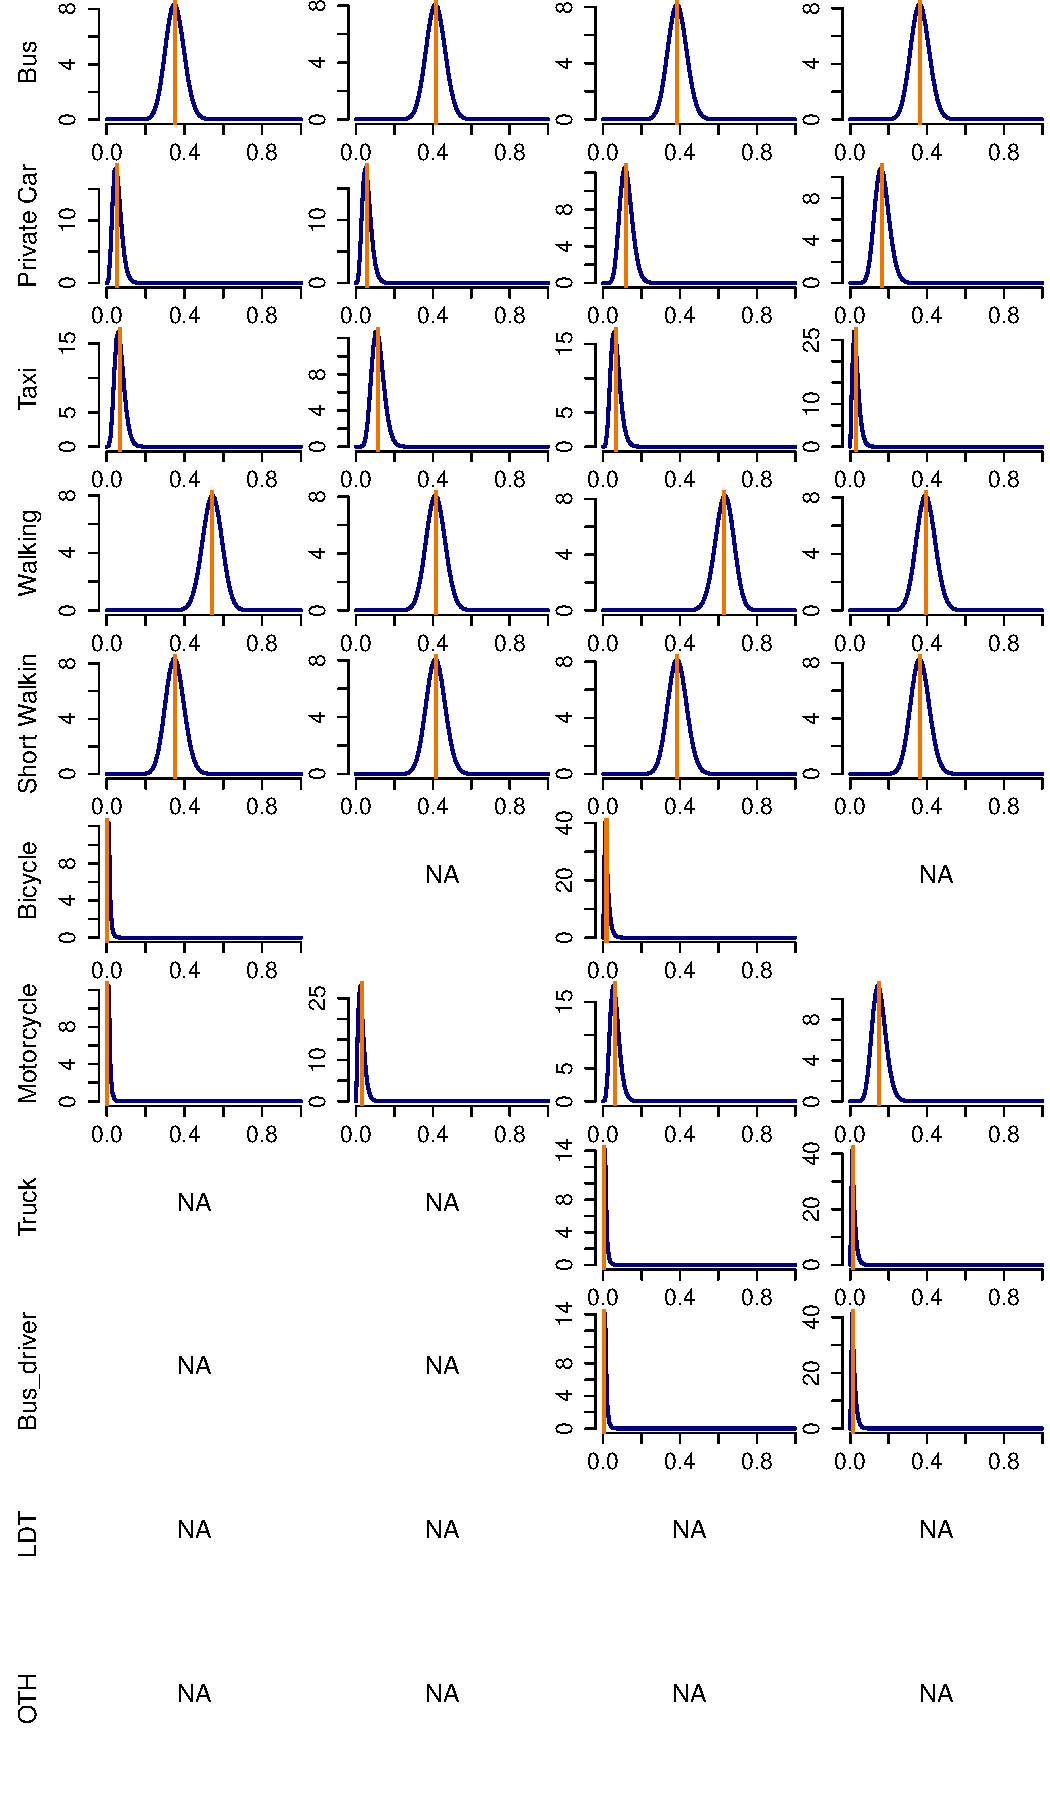
\includegraphics[width=0.7\textwidth]{propensity_to_travel.pdf}
%\caption{\small Distributions for propensities to travel. The propensity is the probability that a member of a demographic group will travel by a particular mode on a particular day. In orange are the raw probabilities based on the synthetic trip set, here shown for the baseline scenario. Beta distributions are defined via a pointiness parameter, set to 100, such that $\alpha+\beta=100$. }
%\label{propensity_to_travel}
%\end{figure}
\begin{figure}[H]
\centering
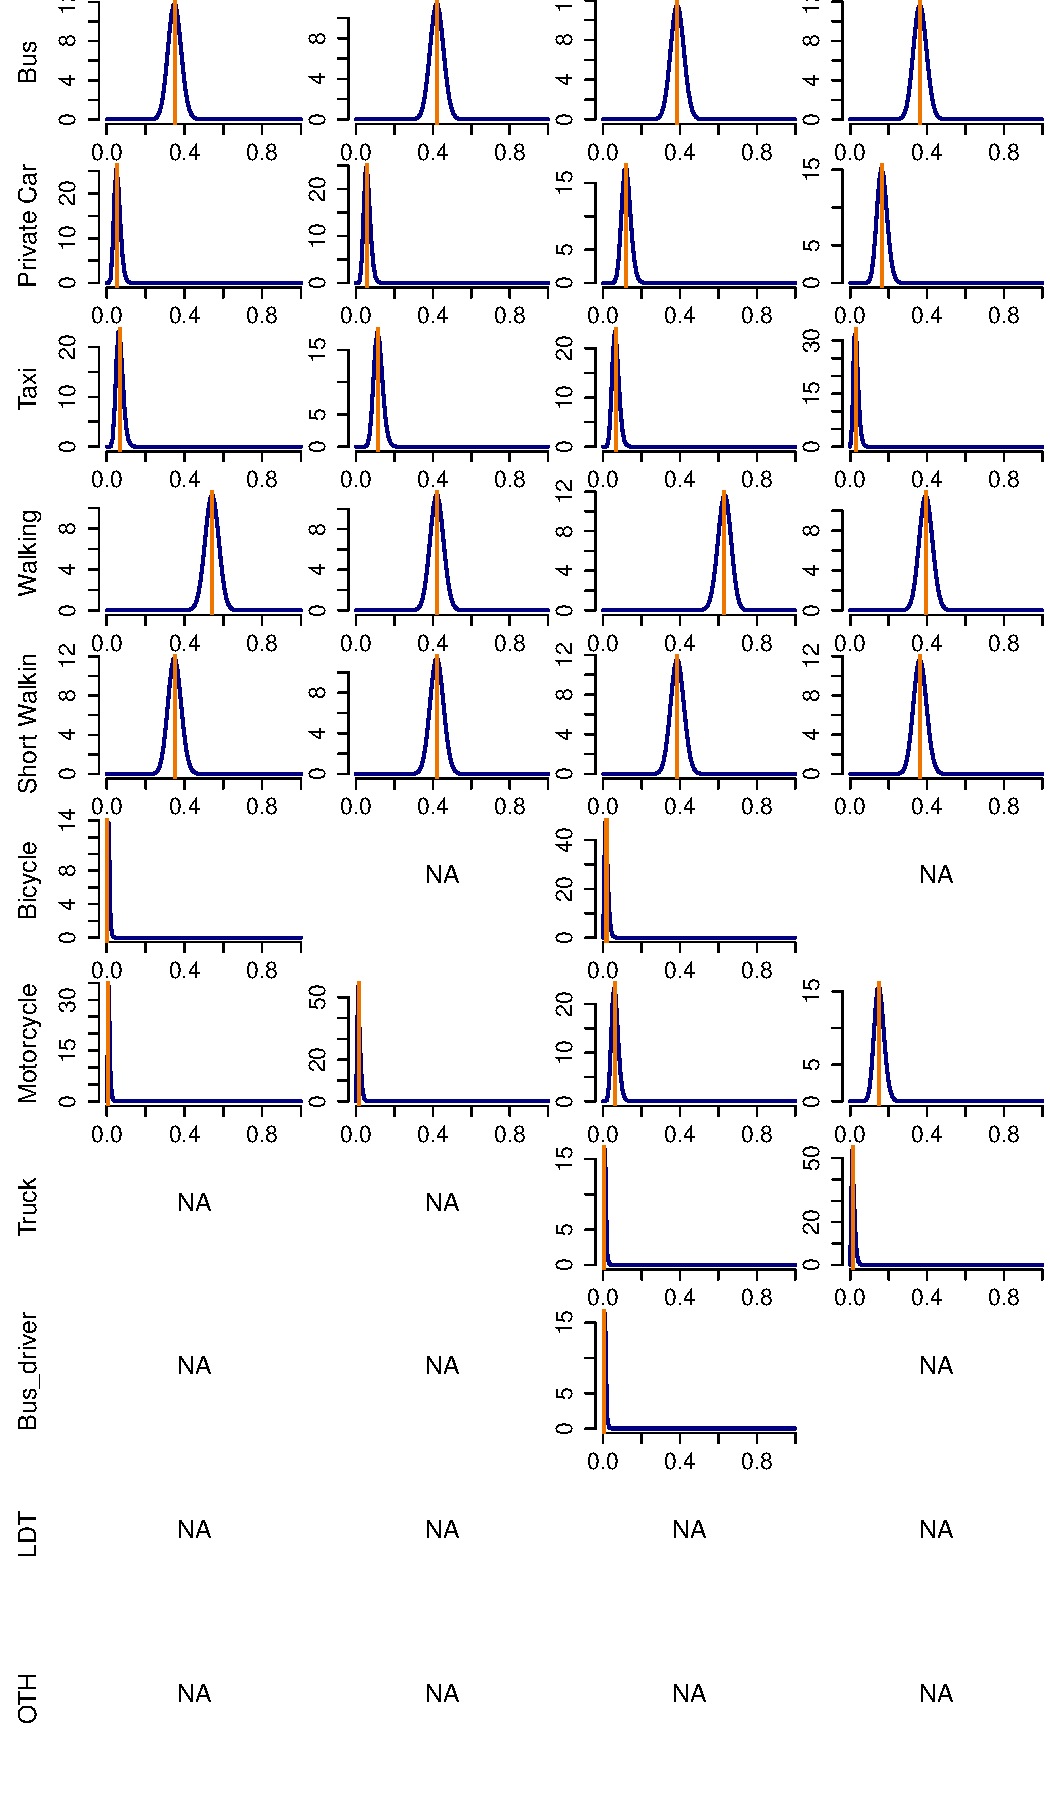
\includegraphics[width=0.7\textwidth]{propensity_to_travel_200.pdf}
\caption{\small Distributions for propensities to travel. The propensity is the probability that a member of a demographic group will travel by a particular mode on a particular day. In orange are the raw probabilities based on the synthetic trip set, here shown for the baseline scenario. Beta distributions are defined via a pointiness parameter, set to 200, such that $\alpha+\beta=200$. }
\label{propensity_to_travel}
\end{figure}

%\begin{comment}
\subsection{Extrapolating to one week of travel}\label{Extrapolation}

%Do we want to extrapolate to one week, or one year? We could feasibly sample one week of trips. One year of trips, however, is likely prohibitively expensive.

In order to extrapolate to one week of travel, we consider ``trips'' only at the stage of scenario generation, and proceed with individual-level statistics. Then, in our synthetic population, we have ``duration travelled per mode'' columns. None of the core ITHIM-R functions will use the ``synthetic trip set''.

To get duration per mode per person, we use, for each demographic-group--mode combination, the probability to travel, and the density of the total duration travelled given that travel occurred. To get from one day to one week, consider two cases: one, each individual follows the same pattern of travel every day. That is, we sample one day's travel and apply it to seven days. Two, each individual follows the travel pattern of their demographic group on each day. That is, we sample seven times from the group's density to make up seven days of travel.%We can then sample, for each individual, the likely number of days travelled out of seven (or 365), and sample the likely duration per day. Their total travel will be the sum of these durations.

%To introduce sampling into the calculation, 
In implementation, we blend individual and group-level travel through a ``repetitiveness'' parameter, $\pi$. Each individual has two travel sets: one from their simulated daily travel pattern, and one from the shared, convolved distribution. These travel sets are weighted by $\pi$ and $1-\pi$, respectively. $\delta_{i,m}$ defines the quantile taken for both the individual density, which is scaled up to one week, and the shared distribution, which  is the convolution of the raw density seven times.\footnote{Using the same random variable for both travel sets increases the variability of the resulting dataset. Conversely, using different random variables would result in more homogenous durations, and fewer zeros.} The densities are shown in Figure \ref{raw_densities}.

\begin{figure}[H]
\centering
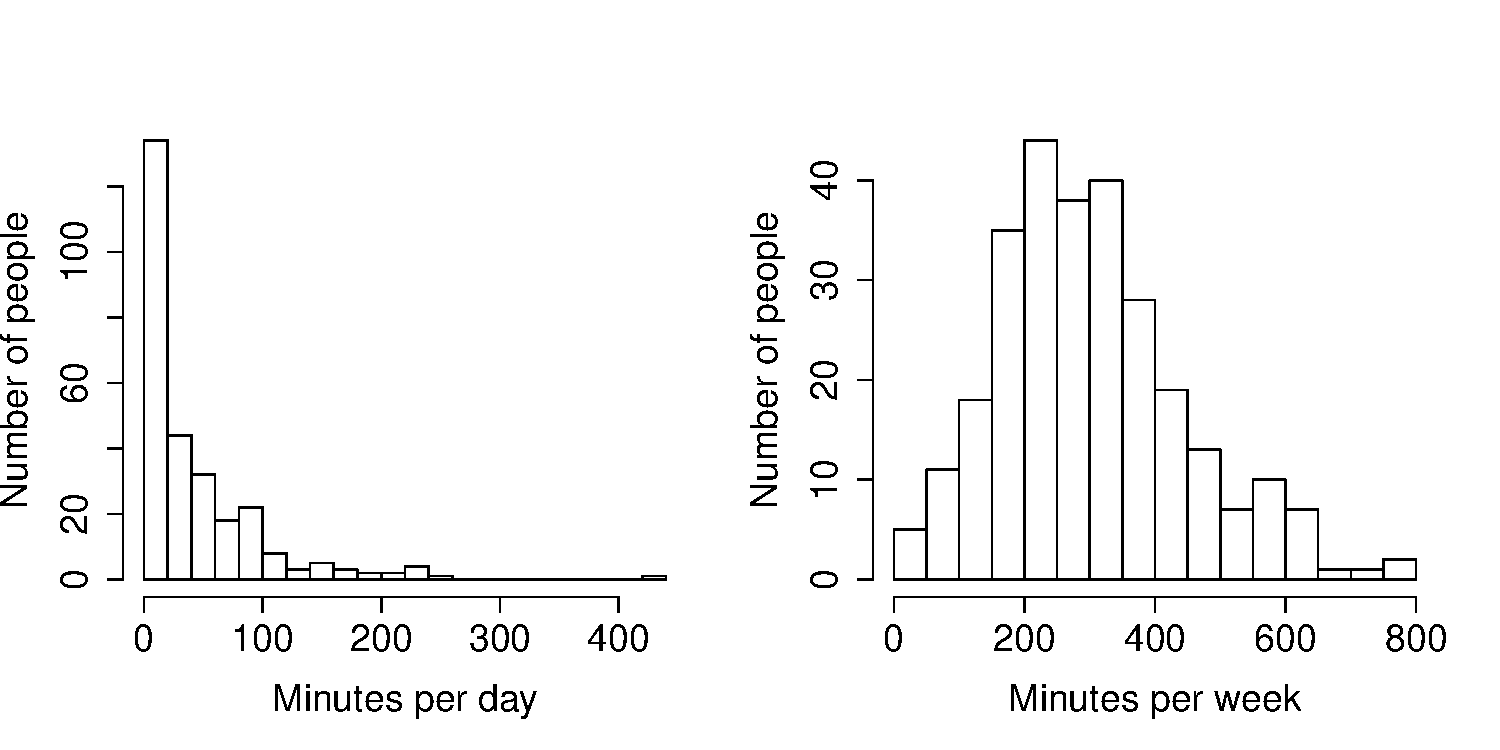
\includegraphics[width=0.8\textwidth]{raw_densities.pdf}
\caption{\small Raw distributions for duration travelled per day (left) from the travel survey. Convolution to one week is shown on the right. We use ````walking'''' mode for demographic group ``Male'', ``15--49''.}
\label{raw_densities}
\end{figure}

%We use the raw density of travel duration per day per mode per demographic group. We can manipulate this density directly, in order to simulate scenarios, or to vary the probability-to-travel parameter, $B_{a,g,m}$. %Note that we are no longer interested in the other parameters of Table \ref{calculations}, and we consider six random variables (five propensities for the five modes, and repetitiveness, $\pi$).
%\end{comment}

\subsection{Simulating a synthetic population}\label{synthpop}

\begin{enumerate}
\item Choose a population size of individuals ${N}$. Label each individual $i=1,...,N$.
\item Allocate each individual to a demographic group according to the proportions in the Accra population (Table \ref{population}). Then each demographic group has number $\tilde{N}_{a,g}$ and  $\sum_{a,g}\tilde{N}_{a,g}=N$.
\item Generate one standard uniform variable per person per mode, $\delta_{i,m}\sim\mathcal{U}(0,1)$. $\delta_{i,m}$ is individual $i$'s propensity to travel by mode $m$. 
\item $\tilde{B}_{a,g,m,s}$ is the propensity of group \{$a,g$\} to travel by mode $m$ in scenario $s$. It is the proportion of raw person--duration values that are zero. It is parametrised by $\alpha_{a,g,m,s}$ and $\beta_{a,g,m,s}$ (Equation \ref{pitilde}). 
\item Let $\mathcal{F}_{a,g,m,s}$ be the raw density for raw person--duration values for demographic group  \{$a,g$\} and mode $m$ in scenario $s$: $\mathcal{F}_{a,g,m,s}=\left\{\sum_{j:i(j)=i,m(j)=m,s(j)=s} T_j\right\}_{i:a(i)=a,g(i)=g}$ i.e. we isolate all individuals $i$ in group $\{a,g\}$ and sum their trip durations by mode $m$ in scenario $s$.% (see Figure \ref{raw_densities}, left).
\item Let $\tilde{\mathcal{F}}_{a,g,m,s}$ be that density corrected to have proportion $\tilde{B}_{a,g,m,s}$ zeros.
%\item Let $\tilde{\mathcal{F}}_{a,g,m,s}^7$ be the week convolution of $\tilde{\mathcal{F}}_{a,g,m,s}$ (see Figure \ref{raw_densities}, right).
\item Define each individual's travel duration as %$D_{i,m,s}=7\pi\cdot\text{CDF}_{\tilde{\mathcal{F}}_{a(i),g(i),m,s}}^{-1}(\delta_{i,m})+(1-\pi)\cdot\text{CDF}_{\tilde{\mathcal{F}}_{a(i),g(i),m,s}^7}^{-1}(\delta_{i,m})$ (see Figure \ref{distances_beta} for resulting distributions).
$D_{i,m,s}=7\cdot\text{CDF}_{\tilde{\mathcal{F}}_{a(i),g(i),m,s}}^{-1}(\delta_{i,m})$ (see Figure \ref{distances_beta} for resulting distributions).
\end{enumerate}

For sampling, we loop over steps 6--7, where each sample has unique $\tilde{B}_{a,g,m,s}$ values. In total, the number of uncertain variables is one per mode. 
%For sampling, we loop over steps 6--8, where each sample has unique $\tilde{B}_{a,g,m,s}$ and $\pi$ values. In total, the number of uncertain variables is one per mode plus one. %Alternatively, we sample a unique $T_j$ set for each iteration similarly to Section \ref{synthtrip},\footnote{For scenario generation, we might want to vary trip duration.} omit step 7, and loop over steps 6, 8 and 9.

\subsection{Simulating a synthetic population with repetitiveness parameter \& uncertain extrapolation}\label{synthpop2}

\begin{enumerate}
\item Choose a population size of individuals ${N}$. Label each individual $i=1,...,N$.
\item Allocate each individual to a demographic group according to the proportions in the Accra population (Table \ref{population}). Then each demographic group has number $\tilde{N}_{a,g}$ and  $\sum_{a,g}\tilde{N}_{a,g}=N$.
\item Generate one standard uniform variable per person per mode, $\delta_{i,m}\sim\mathcal{U}(0,1)$. $\delta_{i,m}$ is individual $i$'s propensity to travel by mode $m$. 
\item $\tilde{B}_{a,g,m,s}$ is the propensity of group \{$a,g$\} to travel by mode $m$ in scenario $s$. It is the proportion of raw person--duration values that are zero. It is parametrised by $\alpha_{a,g,m,s}$ and $\beta_{a,g,m,s}$ (Equation \ref{pitilde}). 
\item Let $\mathcal{F}_{a,g,m,s}$ be the raw density for raw person--duration values for demographic group  \{$a,g$\} and mode $m$ in scenario $s$: $\mathcal{F}_{a,g,m,s}=\left\{\sum_{j:i(j)=i,m(j)=m,s(j)=s} T_j\right\}_{i:a(i)=a,g(i)=g}$ i.e. we isolate all individuals $i$ in group $\{a,g\}$ and sum their trip durations by mode $m$ in scenario $s$.% (see Figure \ref{raw_densities}, left).
%\item Let $\tilde{\mathcal{F}}_{a,g,m,s}$ be that density corrected to have proportion $\tilde{B}_{a,g,m,s}$ zeros.
\item Let $\tilde{\mathcal{F}}_{a,g,m,s}^7$ be the week convolution of $\tilde{\mathcal{F}}_{a,g,m,s}$ (see Figure \ref{raw_densities}, right).
\item Define each individual's travel duration as $D_{i,m,s}=7\pi\cdot\text{CDF}_{\tilde{\mathcal{F}}_{a(i),g(i),m,s}}^{-1}(\delta_{i,m})+(1-\pi)\cdot\text{CDF}_{\tilde{\mathcal{F}}_{a(i),g(i),m,s}^7}^{-1}(\delta_{i,m})$ (see Figure \ref{distances_beta} for resulting distributions).
%$D_{i,m,s}=7\cdot\text{CDF}_{\tilde{\mathcal{F}}_{a(i),g(i),m,s}}^{-1}(\delta_{i,m})$ (see Figure \ref{distances_beta} for resulting distributions).
\end{enumerate}

%For sampling, we loop over steps 6--7, where each sample has unique $\tilde{B}_{a,g,m,s}$ values. In total, the number of uncertain variables is one per mode. 
For sampling, we loop over steps 6--8, where each sample has unique $\tilde{B}_{a,g,m,s}$ and $\pi$ values. In total, the number of uncertain variables is one per mode plus one. %Alternatively, we sample a unique $T_j$ set for each iteration similarly to Section \ref{synthtrip},\footnote{For scenario generation, we might want to vary trip duration.} omit step 7, and loop over steps 6, 8 and 9.






\begin{figure}[h]
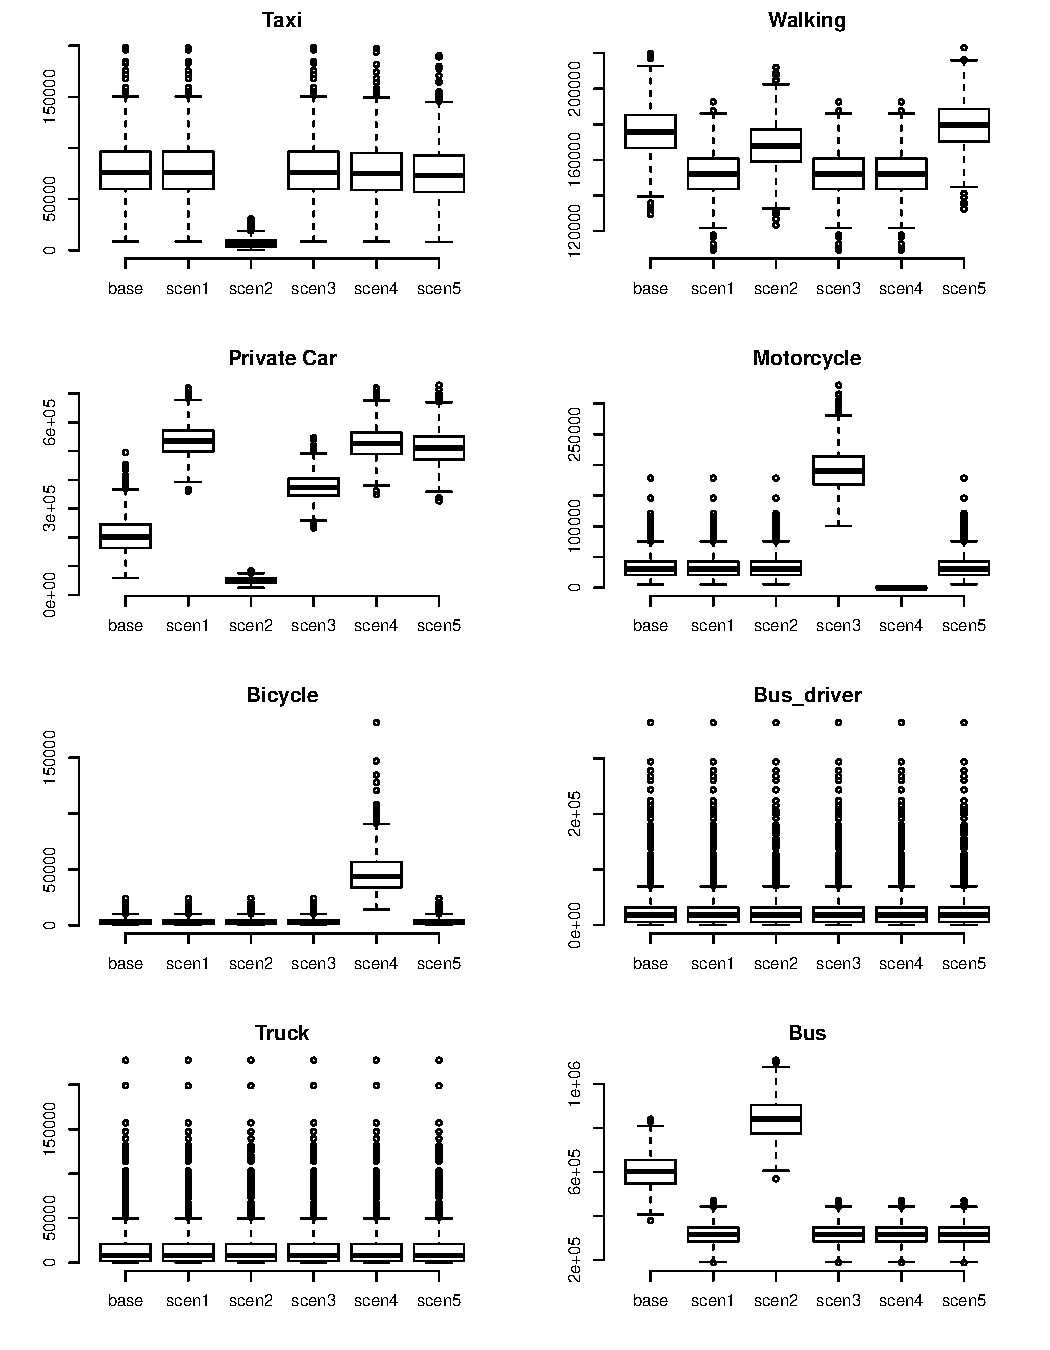
\includegraphics[width=0.8\textwidth]{distances_beta.pdf}
\caption{\small Samples of total distances travelled by mode and scenario.}
\label{distances_beta}
\end{figure}


\clearpage


\subsection{Results}


\begin{figure}[h]
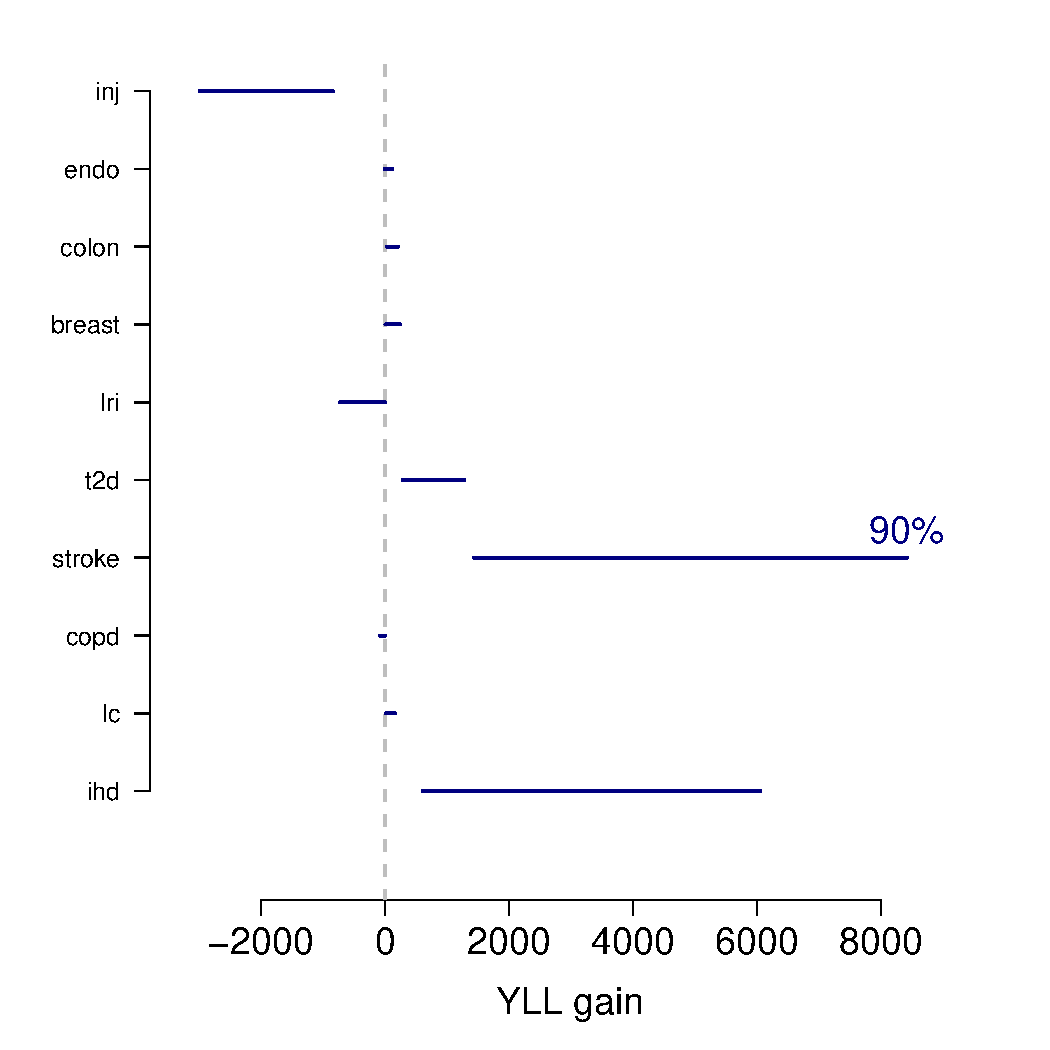
\includegraphics[width=0.8\textwidth]{accra_walk_yll_uncertain_travel.pdf}
\caption{\small YLLs in the scenario minus YLLs in the baseline for Accra, with motorcycle probability scalar 2 in Accra.}
\label{results}
\end{figure}

\begin{figure}[h]
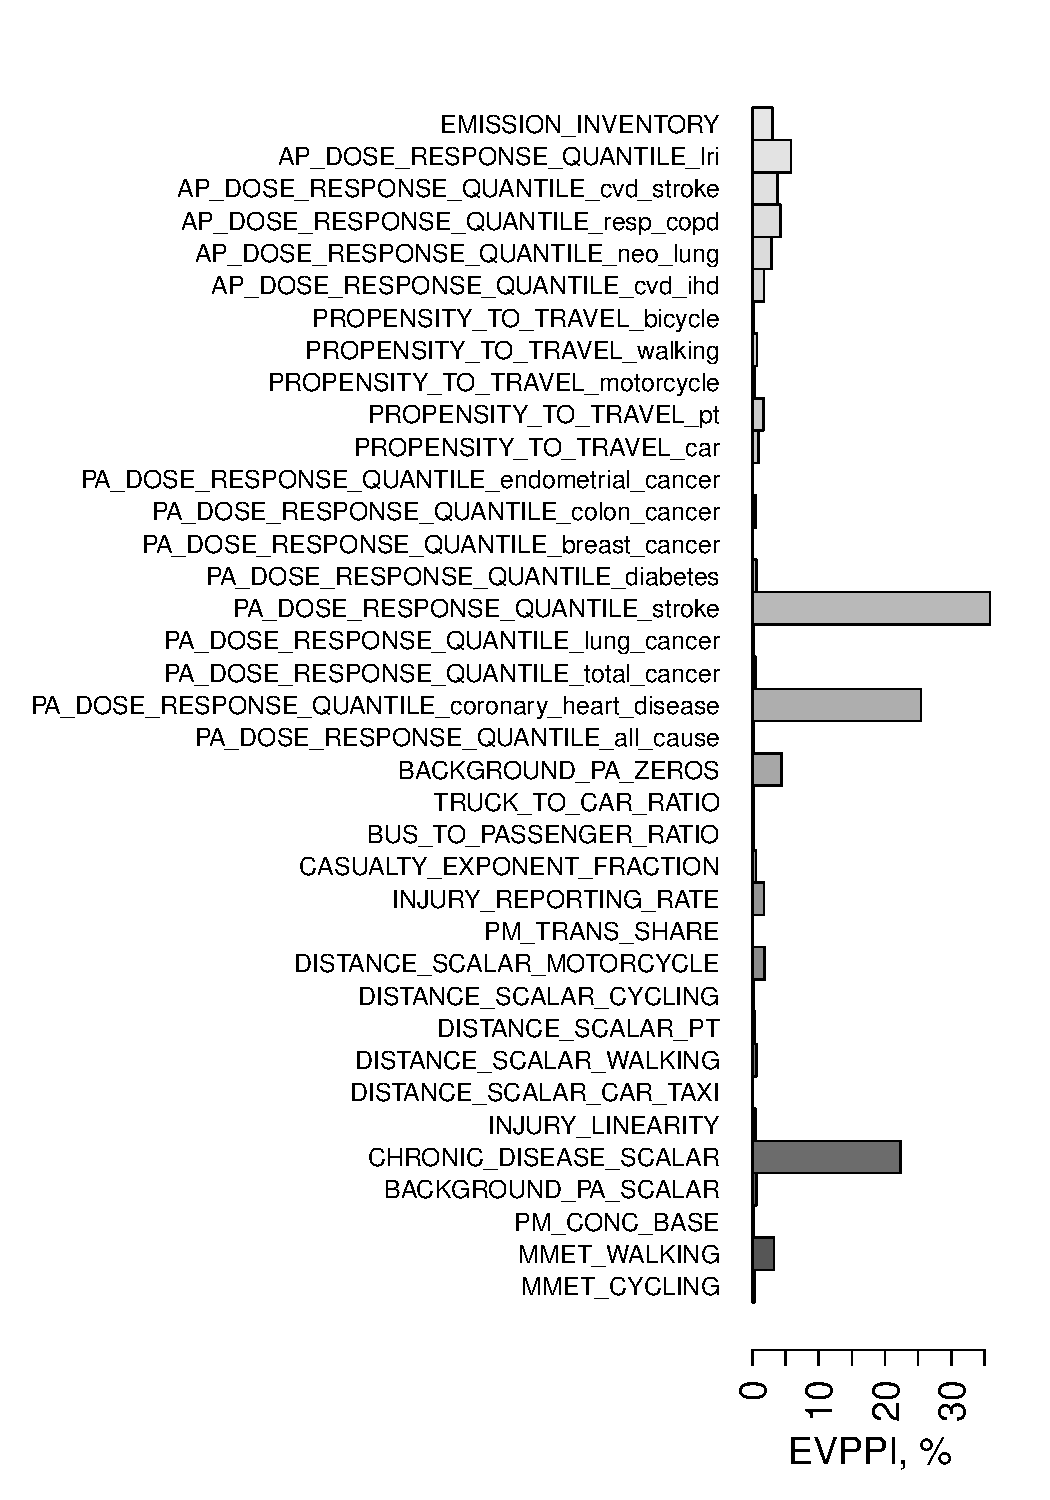
\includegraphics[width=0.7\textwidth]{accra_walk_evppi_uncertain_travel.pdf}
\caption{\small EVPPI for Accra's ``walking'' scenario for all causes of YLLs excluding ``all cause'' and ``neoplasm'', with propensity to motorcycle = 2.}
\label{evppi_mode_propensities_200}
\end{figure}

%\subsection{Questions arising}

%\begin{itemize}
%\item How to model multi-mode trips
%\item Programming: logic of which modes to use
%\item What do we do about zero trips for e.g. older cyclists?
%\item Are bus and truck drivers participants?
%\item Including correlations between modes
%\end{itemize}


\clearpage
\section{Glossary by letter}

\begin{table}[h]
\begin{tabular}{|>{$}r<{$}l|>{$}r<{$}l|>{$}r<{$}l|}
\hline
\text{Letter} & Meaning & \text{Letter} & Meaning & \text{Letter} & Meaning \\
\hline
\alpha &  & a & age & A &  \\
\beta &   & b &   & B & raw travel probabilities \\
\gamma & emission uncertainty  & c &   & C & ventilation constants \\
\delta &  propensity to travel & d & demographic group  & D &  \\
\epsilon & walk-to-bus time  & e &   & E & injury distance exponent \\
\zeta & traffic PM2.5 fraction  & f &   & F & PA DR function \\
\eta & PM2.5 concentration  & g & gender  & G & PA DR curves \\
\theta &  PA uncertainty & h &  disease & H & AP DR curves \\
\iota &   & i &  individual & I & injuries \\
 &   & j & trip  & J &  \\
\kappa & injury regression parameter  & k &   & K & AP exposure \\
\lambda &  travel MMETs & l &   & L &  \\
\mu &  mode distances & m & mode  & M & MMETs per person \\
\nu &   & n &   & N & population \\
\xi &  AP DR quantile & o & outcome  & O &  \\
\pi & travel repetitiveness  & p &   & P & vehicle emissions \\
 &   & q &   & Q &  person weights \\
\rho & chronic disease scalar  & r &   & R & death-to-injury ratio \\
\sigma & injury reporting rate  & s & scenario  & S &  \\
\tau &   & t &   & T & trips \\
\upsilon &   & u &   & U & burden of disease \\
\phi & PA DR quantile  & v &   & V & AP per person \\
 &   & w & AP DR parameter   & W & relative risks \\
\chi & day-to-week travel scalar  & x & PA DR parameter  & X & injury model matrix \\
\psi & casualty fraction of $\omega$  & y & year & Y & individual MMETs \\
\omega & sum of distance exponents  & z & PA dose  & Z & speeds \\
\hline
\end{tabular}
\end{table}


\end{appendix}
\clearpage
\bibliographystyle{agsm}
\bibliography{ithim}
\end{document}


\clearpage
\section{Injury model}

\subsection{Basic set up}

We begin with the trip set, $T_j$. There is one value (a distance) per trip $j$. $T_j$ is informed by a set of covariates $z=\{a,g,m\}$. $a$ is the age of the person who took the trip, $g$ their gender, and $m$ the mode. The complete set $M$ is the set of all the unique modes $m$ in the trip set $T_j$.

From $T_j$ we calculate the total distance per set $x\in X$: $$D_x=\sum_{j:z_j= x}T_j.$$ $X$ is the complete set of all unique combinations of the variables $z$.

We augment $D_X$ with distances from modes not included in the trip set. We denote the augmented set of modes $M^+$ and the augmented distance set $D_{X^+}$.

For each mode in $M^+$ we calculate the total distance travelled as $$\hat{D}_{m}=\sum_{a,g}D_{a,g,m}.$$ 

We define a set $y=\{a',g',m'\}$ analogous to $x$, so that they each represent one party in a collision/encounter. Then the injury set is defined as $I_{x,y}$. From this we calculate rates of injury as $$R_{x,y}=\frac{I_{x,y} \sqrt{\hat{D}_m\hat{D}_{m'}}}{D_xD_y}.$$

\subsection{Multinational}

We can add/subtract covariates to/from $x$ and $y$ in the above framework. For example, we can include the country, $c$, as in Figure \ref{plate}.

\begin{figure}[h]
  \centering
  \tikz{ %
    \node[latent] (sigD) {$\sigma_x^{(D)}$} ; %
    \node[latent, right=of sigD] (D0) {$D_x^{(0)}$} ; %
    \node[latent, right=of D0] (R0) {$R_{x,y}^{(0)}$} ; %
    \node[latent, right=of R0] (sigR) {$\sigma_{x,y}^{(R)}$} ; %
    \node[latent, below=of D0] (mux) {$\mu_{x,c}$} ; %
    \node[latent, below=of mux] (Dx) {$D_{x,c}$} ; %
    \node[latent, left=of mux] (lambda) {$\lambda_{x,c}$} ; %
    \node[latent, left=of lambda,xshift=-1cm] (lambda0) {$\lambda_{x}^{(0)}$} ; %
    \node[latent, below=of R0] (Rxy) {$R_{x,y,c}$} ; %
    \node[obs, below=of lambda] (T) {$T_{j,c}$} ; %
    \node[obs, below=of Rxy] (I) {$I_{x,y,c}$} ; %
    \plate[inner sep=0.25cm, yshift=0.12cm] {plateT} {(T)} {$j=1,...,J$}; %
    \plate[inner sep=0.25cm, yshift=0.12cm] {plate1} {(lambda) (plateT) (I)} {$c=1,...,C$}; %
    \edge {sigD,D0} {mux} ; %
    \edge {mux,lambda} {Dx} ; %
    \edge {sigR,R0} {Rxy} ; %
    \edge {mux,lambda} {T} ; %
    \edge {lambda0} {lambda} ; %
    \edge {Dx,Rxy} {I} ; %
  }
  \caption{\small Plate diagram relating latent distance and rate distributions to observed travel surveys and injuries. This diagram could be a single set $\{x,y\}$ or it could represent the joint distributions for all $\{x,y\}$. $D_x^{(0)}$ is the distance distribution for covariates $x$, and is described with a log-normal distribution. $R_{x,y}^{(0)}$ is the rate distribution for collision between covariates $x$ and $y$ and can also be log-normally distributed. $\sigma_x^{(D)}$ and $\sigma_{x,y}^{(R)}$ are the inter-country variability for distances and rates, respectively. We might want to impose that $\sigma_x^{(D)}>\sigma_{x,y}^{(R)}$? Then $\mu_{x,c}|D_x^{(0)},\sigma_x^{(D)}$ and $R_{x,y,c}|R_{x,y}^{(0)},\sigma_{x,y}^{(R)}$ can be log-normally distributed. $\lambda_{x,c}$ is a zero-inflated Poisson distribution counting the number of trips per person for covariates $x$, so $D_{x,c}|\mu_{x,c},\lambda_{x,c}$ is a compound Poisson log-normal distribution.  $I_{x,y,c}|D_{x,c},R_{x,y,c}$ is Poisson distributed, and $T_{j,c}|D_{x,c}$ would be a non-summed compound Poisson log-normal distribution.}
\label{plate}
\end{figure}
\begin{figure}[h]
  \centering
  \tikz{ %
    \node[latent] (sigD) {$\sigma_x^{(D)}$} ; %
    \node[latent, right=of sigD] (D0) {$D_x^{(0)}$} ; %
    \node[latent, right=of D0] (R0) {$R_{x,y}^{(0)}$} ; %
    \node[latent, right=of R0] (sigR) {$\sigma_{x,y}^{(R)}$} ; %
    \node[latent, below=of D0] (mux) {$\mu_{x,c}$} ; %
    \node[latent, below=of mux] (Dx) {$D_{x,c}$} ; %
    \node[latent, left=of mux] (lambda) {$\lambda_{x,c}$} ; %
    \node[latent, left=of lambda,xshift=-1cm] (lambda0) {$\lambda_{x}^{(0)}$} ; %
    \node[latent, below=of R0] (Rxy) {$R_{x,y,c}$} ; %
    \node[obs, below=of lambda] (T) {$T_{j,c}$} ; %
    \node[obs, below=of Rxy] (I) {$I_{x,y,c}$} ; %
    \plate[inner sep=0.25cm, yshift=0.12cm] {plateT} {(T)} {$j=1,...,J$}; %
    \edge {sigD,D0} {mux} ; %
    \edge {mux,lambda} {Dx} ; %
    \edge {sigR,R0} {Rxy} ; %
    \edge {mux,lambda} {T} ; %
    \edge {lambda0} {lambda} ; %
    \node[latent, below=of Rxy] (I) {$I_{x,y,c}$} ; %
    \node[obs, below=of I] (Ixc) {$\hat{I}_{x,c}$} ; %
    \plate[inner sep=0.25cm, yshift=0.12cm] {plate1} {(mux) (plateT) (Ixc)} {$c=1,...,C$}; %
    \edge {I} {Ixc} ; %
    \edge {Dx,Rxy} {I} ; %
  }
  \caption{\small Question: can we combine the model in Figure \ref{plate} with the case where we are missing some information in the injuries? Suppose, for example, that we don't have the details of the other vehicle ($y$), only the sum $\hat{I}_{x,c}=\sum_yI_{x,y,c}$}
\label{plate2}
\end{figure}
